\chapter{Experiments}
\label{ch:experiments}

Our goal is simulating different strategies of online learning for the new web
interface. Before we can do that, we first pre-train parsers in
Section~\ref{sec:pre-training} on the existing datasets \nlmapstwo{} and the
variations we introduced in \nlmapsthree{} and evaluate whether the dataset
extensions yield any improvement in parser quality. In
Section~\ref{sec:annotation}, we then hire annotators to use our web interface
to ask NL queries and correct the MRL parse if it is incorrect, thus collecting
a new dataset consisting of real user queries. Finally, in
Section~\ref{sec:online-simulation} we use the newly acquired dataset for
evaluating various online learning setups.

For all our experiments, we use the same model architecture: A character-based
one-layer bidirectional GRU encoder-decoder \parencite{cho-2014} model with
attention.\parencite{bahdanau-2015} The dimension of both source and target
embeddings is 620, the encoder layer size is 500, the decoder layer size is 1000
and we don’t use dropout. This model configuration is adopted from
\textcite{staniek-2020}.

\section{Training on \nlmapstwo{} and \nlmapsthree{}}
\label{sec:pre-training}

While \textcite{staniek-2020} trained his model on the \nlmapstwo{} dataset for
100 epochs (of 16172 instances each), we train our models in this section for a
shorter time, which is still enough for sufficient convergence: The model on
\nlmapstwoone{} is trained for 60 epochs (of 15113 instances each), while the
models on variations of \nlmapsthree{} are trained for 30 epochs (of 30226
instances each). All models are trained with the Adam optimizer (\(\beta_1 =
0.9\) and \(\beta_2 = 0.999\)) and a learning rate of \num{0.0002}

Table~\ref{tab:pre-trained-performance} shows the results of testing the models
on the different variations of \nlmaps{} datasets. Recall: \nlmtwoone{} is the
result of fixing issues in the MRL queries of \nlmtwo{}, but has identical NL
queries; \nlmthreea{} is purely generated with probabilistic templates and
\nlmthreeb{} is its counterpart with added noise; \nlmthreenormal{} is
\nlmtwoone{} + \nlmthreea{} and \nlmthree{} is \nlmtwoone{} + \nlmthreeb{}. The
datasets \nlmfourraw{} and \nlmfour{} are introduced in
Section~\ref{sec:annotation} and are the user-supplied MRL-NL pairs with some
corrections applied to them in \nlmfour{}. Even though the last two datasets
were not yet available when the models were pre-trained, we still evaluate the
pre-trained models on them in this section because we consider the results on
these user-supplied queries the most relevant.

\begin{table}[h]
  \centering
  \begin{tabular}{lcccccccc}
    \toprule
    \diagbox{Train}{Test} & \nlmtwo{} & \nlmtwoone{} & \nlmthreea{} & \nlmthreeb{} & \nlmthreenormal{} & \nlmthree{} & \nlmfourraw{} & \nlmfour{}\\
    \midrule
    \textcite{staniek-2020} & \bfnum{0.898} & \num{0.844} & \num{0.039} & \num{0.033} & \num{0.441} & \num{0.439} & \num{0.050} & \num{0.052}\\
    \nlmtwoone{} & \num{0.783} & \num{0.913} & \num{0.034} & \num{0.029} & \num{0.474} & \num{0.471} & \num{0.070} & \num{0.069}\\
    \nlmthreea{} & \num{0.224} & \num{0.251} & \bfnum{0.987} & \num{0.789} & \num{0.618} & \num{0.519} & \num{0.217} & \num{0.223}\\
    \nlmthreeb{} & \num{0.372} & \num{0.424} & \num{0.976} & \bfnum{0.884} & \num{0.700} & \num{0.656} & \num{0.226} & \num{0.233}\\
    \nlmthreenormal{} & \num{0.790} & \bfnum{0.919} & \num{0.978} & \num{0.792} & \bfnum{0.948} & \num{0.857} & \bfnum{0.307} & \bfnum{0.311}\\
    \nlmthree{} & \num{0.787} & \num{0.913} & \num{0.950} & \num{0.834} & \num{0.931} & \bfnum{0.874} & \num{0.281} & \num{0.289}\\
    \bottomrule
  \end{tabular}
  \caption{Performance of pre-trained parsers}
  \label{tab:pre-trained-performance}
\end{table}

Unsurprisingly, the model by \textcite{staniek-2020}, which was trained on
\nlmapstwo{}, performs best on the corresponding test set with an accuracy of
\SI{89.8}{\%}. The model trained on \nlmtwoone{}, which contains the fixes of
tag usage and inconsistencies described in Chapter~\ref{ch:nlmaps-improvement},
achieves a higher accuracy on its corresponding test set with \SI{91.3}{\%}.
This is to be expected since the resolution of inconsistencies in MRL structure
and tag usage makes a new part of the dataset accessible for confident
predictions in the first place. These two models’ performance drops dramatically
on new datasets. An error analysis (see Figure~\ref{fig:v21-errors}) shows that
not only does the model trained on \nlmtwoone{} make an error in the
\mrl{target_nwr} operator in over \SI{70}{\%} of queries from the \nlmapsfour{}
test set, the recognized \mrl{area} is false in more than half the queries, as
well.

\begin{figure}[h]
  \centering
  \resizebox{\textwidth}{!}{%% Creator: Matplotlib, PGF backend
%%
%% To include the figure in your LaTeX document, write
%%   \input{<filename>.pgf}
%%
%% Make sure the required packages are loaded in your preamble
%%   \usepackage{pgf}
%%
%% and, on pdftex
%%   \usepackage[utf8]{inputenc}\DeclareUnicodeCharacter{2212}{-}
%%
%% or, on luatex and xetex
%%   \usepackage{unicode-math}
%%
%% Figures using additional raster images can only be included by \input if
%% they are in the same directory as the main LaTeX file. For loading figures
%% from other directories you can use the `import` package
%%   \usepackage{import}
%%
%% and then include the figures with
%%   \import{<path to file>}{<filename>.pgf}
%%
%% Matplotlib used the following preamble
%%   \usepackage{fontspec}
%%   \setmainfont{LinLibertine_R.otf}[Path=/usr/share/texmf-dist/fonts/opentype/public/libertine/]
%%   \setsansfont{LinLibertine_R.otf}[Path=/usr/share/texmf-dist/fonts/opentype/public/libertine/]
%%   \setmonofont{DejaVuSansMono.ttf}[Path=/home/gorgor/.virtualenvs/ma/lib/python3.9/site-packages/matplotlib/mpl-data/fonts/ttf/]
%%
\begingroup%
\makeatletter%
\begin{pgfpicture}%
\pgfpathrectangle{\pgfpointorigin}{\pgfqpoint{6.400000in}{3.500000in}}%
\pgfusepath{use as bounding box, clip}%
\begin{pgfscope}%
\pgfsetbuttcap%
\pgfsetmiterjoin%
\definecolor{currentfill}{rgb}{1.000000,1.000000,1.000000}%
\pgfsetfillcolor{currentfill}%
\pgfsetlinewidth{0.000000pt}%
\definecolor{currentstroke}{rgb}{1.000000,1.000000,1.000000}%
\pgfsetstrokecolor{currentstroke}%
\pgfsetdash{}{0pt}%
\pgfpathmoveto{\pgfqpoint{0.000000in}{0.000000in}}%
\pgfpathlineto{\pgfqpoint{6.400000in}{0.000000in}}%
\pgfpathlineto{\pgfqpoint{6.400000in}{3.500000in}}%
\pgfpathlineto{\pgfqpoint{0.000000in}{3.500000in}}%
\pgfpathclose%
\pgfusepath{fill}%
\end{pgfscope}%
\begin{pgfscope}%
\pgfsetbuttcap%
\pgfsetmiterjoin%
\definecolor{currentfill}{rgb}{1.000000,1.000000,1.000000}%
\pgfsetfillcolor{currentfill}%
\pgfsetlinewidth{0.000000pt}%
\definecolor{currentstroke}{rgb}{0.000000,0.000000,0.000000}%
\pgfsetstrokecolor{currentstroke}%
\pgfsetstrokeopacity{0.000000}%
\pgfsetdash{}{0pt}%
\pgfpathmoveto{\pgfqpoint{1.024000in}{0.490000in}}%
\pgfpathlineto{\pgfqpoint{6.272000in}{0.490000in}}%
\pgfpathlineto{\pgfqpoint{6.272000in}{3.430000in}}%
\pgfpathlineto{\pgfqpoint{1.024000in}{3.430000in}}%
\pgfpathclose%
\pgfusepath{fill}%
\end{pgfscope}%
\begin{pgfscope}%
\pgfpathrectangle{\pgfqpoint{1.024000in}{0.490000in}}{\pgfqpoint{5.248000in}{2.940000in}}%
\pgfusepath{clip}%
\pgfsetbuttcap%
\pgfsetmiterjoin%
\definecolor{currentfill}{rgb}{1.000000,0.000000,0.000000}%
\pgfsetfillcolor{currentfill}%
\pgfsetlinewidth{0.000000pt}%
\definecolor{currentstroke}{rgb}{0.000000,0.000000,0.000000}%
\pgfsetstrokecolor{currentstroke}%
\pgfsetstrokeopacity{0.000000}%
\pgfsetdash{}{0pt}%
\pgfpathmoveto{\pgfqpoint{1.024000in}{0.623636in}}%
\pgfpathlineto{\pgfqpoint{1.997139in}{0.623636in}}%
\pgfpathlineto{\pgfqpoint{1.997139in}{0.829231in}}%
\pgfpathlineto{\pgfqpoint{1.024000in}{0.829231in}}%
\pgfpathclose%
\pgfusepath{fill}%
\end{pgfscope}%
\begin{pgfscope}%
\pgfpathrectangle{\pgfqpoint{1.024000in}{0.490000in}}{\pgfqpoint{5.248000in}{2.940000in}}%
\pgfusepath{clip}%
\pgfsetbuttcap%
\pgfsetmiterjoin%
\definecolor{currentfill}{rgb}{1.000000,0.000000,0.000000}%
\pgfsetfillcolor{currentfill}%
\pgfsetlinewidth{0.000000pt}%
\definecolor{currentstroke}{rgb}{0.000000,0.000000,0.000000}%
\pgfsetstrokecolor{currentstroke}%
\pgfsetstrokeopacity{0.000000}%
\pgfsetdash{}{0pt}%
\pgfpathmoveto{\pgfqpoint{1.024000in}{1.034825in}}%
\pgfpathlineto{\pgfqpoint{1.322893in}{1.034825in}}%
\pgfpathlineto{\pgfqpoint{1.322893in}{1.240420in}}%
\pgfpathlineto{\pgfqpoint{1.024000in}{1.240420in}}%
\pgfpathclose%
\pgfusepath{fill}%
\end{pgfscope}%
\begin{pgfscope}%
\pgfpathrectangle{\pgfqpoint{1.024000in}{0.490000in}}{\pgfqpoint{5.248000in}{2.940000in}}%
\pgfusepath{clip}%
\pgfsetbuttcap%
\pgfsetmiterjoin%
\definecolor{currentfill}{rgb}{1.000000,0.000000,0.000000}%
\pgfsetfillcolor{currentfill}%
\pgfsetlinewidth{0.000000pt}%
\definecolor{currentstroke}{rgb}{0.000000,0.000000,0.000000}%
\pgfsetstrokecolor{currentstroke}%
\pgfsetstrokeopacity{0.000000}%
\pgfsetdash{}{0pt}%
\pgfpathmoveto{\pgfqpoint{1.024000in}{1.446014in}}%
\pgfpathlineto{\pgfqpoint{1.128265in}{1.446014in}}%
\pgfpathlineto{\pgfqpoint{1.128265in}{1.651608in}}%
\pgfpathlineto{\pgfqpoint{1.024000in}{1.651608in}}%
\pgfpathclose%
\pgfusepath{fill}%
\end{pgfscope}%
\begin{pgfscope}%
\pgfpathrectangle{\pgfqpoint{1.024000in}{0.490000in}}{\pgfqpoint{5.248000in}{2.940000in}}%
\pgfusepath{clip}%
\pgfsetbuttcap%
\pgfsetmiterjoin%
\definecolor{currentfill}{rgb}{1.000000,0.000000,0.000000}%
\pgfsetfillcolor{currentfill}%
\pgfsetlinewidth{0.000000pt}%
\definecolor{currentstroke}{rgb}{0.000000,0.000000,0.000000}%
\pgfsetstrokecolor{currentstroke}%
\pgfsetstrokeopacity{0.000000}%
\pgfsetdash{}{0pt}%
\pgfpathmoveto{\pgfqpoint{1.024000in}{1.857203in}}%
\pgfpathlineto{\pgfqpoint{4.833144in}{1.857203in}}%
\pgfpathlineto{\pgfqpoint{4.833144in}{2.062797in}}%
\pgfpathlineto{\pgfqpoint{1.024000in}{2.062797in}}%
\pgfpathclose%
\pgfusepath{fill}%
\end{pgfscope}%
\begin{pgfscope}%
\pgfpathrectangle{\pgfqpoint{1.024000in}{0.490000in}}{\pgfqpoint{5.248000in}{2.940000in}}%
\pgfusepath{clip}%
\pgfsetbuttcap%
\pgfsetmiterjoin%
\definecolor{currentfill}{rgb}{1.000000,0.000000,0.000000}%
\pgfsetfillcolor{currentfill}%
\pgfsetlinewidth{0.000000pt}%
\definecolor{currentstroke}{rgb}{0.000000,0.000000,0.000000}%
\pgfsetstrokecolor{currentstroke}%
\pgfsetstrokeopacity{0.000000}%
\pgfsetdash{}{0pt}%
\pgfpathmoveto{\pgfqpoint{1.024000in}{2.268392in}}%
\pgfpathlineto{\pgfqpoint{1.510570in}{2.268392in}}%
\pgfpathlineto{\pgfqpoint{1.510570in}{2.473986in}}%
\pgfpathlineto{\pgfqpoint{1.024000in}{2.473986in}}%
\pgfpathclose%
\pgfusepath{fill}%
\end{pgfscope}%
\begin{pgfscope}%
\pgfpathrectangle{\pgfqpoint{1.024000in}{0.490000in}}{\pgfqpoint{5.248000in}{2.940000in}}%
\pgfusepath{clip}%
\pgfsetbuttcap%
\pgfsetmiterjoin%
\definecolor{currentfill}{rgb}{1.000000,0.000000,0.000000}%
\pgfsetfillcolor{currentfill}%
\pgfsetlinewidth{0.000000pt}%
\definecolor{currentstroke}{rgb}{0.000000,0.000000,0.000000}%
\pgfsetstrokecolor{currentstroke}%
\pgfsetstrokeopacity{0.000000}%
\pgfsetdash{}{0pt}%
\pgfpathmoveto{\pgfqpoint{1.024000in}{2.679580in}}%
\pgfpathlineto{\pgfqpoint{3.790495in}{2.679580in}}%
\pgfpathlineto{\pgfqpoint{3.790495in}{2.885175in}}%
\pgfpathlineto{\pgfqpoint{1.024000in}{2.885175in}}%
\pgfpathclose%
\pgfusepath{fill}%
\end{pgfscope}%
\begin{pgfscope}%
\pgfpathrectangle{\pgfqpoint{1.024000in}{0.490000in}}{\pgfqpoint{5.248000in}{2.940000in}}%
\pgfusepath{clip}%
\pgfsetbuttcap%
\pgfsetmiterjoin%
\definecolor{currentfill}{rgb}{1.000000,0.000000,0.000000}%
\pgfsetfillcolor{currentfill}%
\pgfsetlinewidth{0.000000pt}%
\definecolor{currentstroke}{rgb}{0.000000,0.000000,0.000000}%
\pgfsetstrokecolor{currentstroke}%
\pgfsetstrokeopacity{0.000000}%
\pgfsetdash{}{0pt}%
\pgfpathmoveto{\pgfqpoint{1.024000in}{3.090769in}}%
\pgfpathlineto{\pgfqpoint{1.872021in}{3.090769in}}%
\pgfpathlineto{\pgfqpoint{1.872021in}{3.296364in}}%
\pgfpathlineto{\pgfqpoint{1.024000in}{3.296364in}}%
\pgfpathclose%
\pgfusepath{fill}%
\end{pgfscope}%
\begin{pgfscope}%
\pgfpathrectangle{\pgfqpoint{1.024000in}{0.490000in}}{\pgfqpoint{5.248000in}{2.940000in}}%
\pgfusepath{clip}%
\pgfsetbuttcap%
\pgfsetmiterjoin%
\definecolor{currentfill}{rgb}{0.756863,0.988235,0.756863}%
\pgfsetfillcolor{currentfill}%
\pgfsetlinewidth{0.000000pt}%
\definecolor{currentstroke}{rgb}{0.000000,0.000000,0.000000}%
\pgfsetstrokecolor{currentstroke}%
\pgfsetstrokeopacity{0.000000}%
\pgfsetdash{}{0pt}%
\pgfpathmoveto{\pgfqpoint{1.997139in}{0.623636in}}%
\pgfpathlineto{\pgfqpoint{6.272000in}{0.623636in}}%
\pgfpathlineto{\pgfqpoint{6.272000in}{0.829231in}}%
\pgfpathlineto{\pgfqpoint{1.997139in}{0.829231in}}%
\pgfpathclose%
\pgfusepath{fill}%
\end{pgfscope}%
\begin{pgfscope}%
\pgfpathrectangle{\pgfqpoint{1.024000in}{0.490000in}}{\pgfqpoint{5.248000in}{2.940000in}}%
\pgfusepath{clip}%
\pgfsetbuttcap%
\pgfsetmiterjoin%
\definecolor{currentfill}{rgb}{0.756863,0.988235,0.756863}%
\pgfsetfillcolor{currentfill}%
\pgfsetlinewidth{0.000000pt}%
\definecolor{currentstroke}{rgb}{0.000000,0.000000,0.000000}%
\pgfsetstrokecolor{currentstroke}%
\pgfsetstrokeopacity{0.000000}%
\pgfsetdash{}{0pt}%
\pgfpathmoveto{\pgfqpoint{1.322893in}{1.034825in}}%
\pgfpathlineto{\pgfqpoint{6.272000in}{1.034825in}}%
\pgfpathlineto{\pgfqpoint{6.272000in}{1.240420in}}%
\pgfpathlineto{\pgfqpoint{1.322893in}{1.240420in}}%
\pgfpathclose%
\pgfusepath{fill}%
\end{pgfscope}%
\begin{pgfscope}%
\pgfpathrectangle{\pgfqpoint{1.024000in}{0.490000in}}{\pgfqpoint{5.248000in}{2.940000in}}%
\pgfusepath{clip}%
\pgfsetbuttcap%
\pgfsetmiterjoin%
\definecolor{currentfill}{rgb}{0.756863,0.988235,0.756863}%
\pgfsetfillcolor{currentfill}%
\pgfsetlinewidth{0.000000pt}%
\definecolor{currentstroke}{rgb}{0.000000,0.000000,0.000000}%
\pgfsetstrokecolor{currentstroke}%
\pgfsetstrokeopacity{0.000000}%
\pgfsetdash{}{0pt}%
\pgfpathmoveto{\pgfqpoint{1.128265in}{1.446014in}}%
\pgfpathlineto{\pgfqpoint{6.272000in}{1.446014in}}%
\pgfpathlineto{\pgfqpoint{6.272000in}{1.651608in}}%
\pgfpathlineto{\pgfqpoint{1.128265in}{1.651608in}}%
\pgfpathclose%
\pgfusepath{fill}%
\end{pgfscope}%
\begin{pgfscope}%
\pgfpathrectangle{\pgfqpoint{1.024000in}{0.490000in}}{\pgfqpoint{5.248000in}{2.940000in}}%
\pgfusepath{clip}%
\pgfsetbuttcap%
\pgfsetmiterjoin%
\definecolor{currentfill}{rgb}{0.756863,0.988235,0.756863}%
\pgfsetfillcolor{currentfill}%
\pgfsetlinewidth{0.000000pt}%
\definecolor{currentstroke}{rgb}{0.000000,0.000000,0.000000}%
\pgfsetstrokecolor{currentstroke}%
\pgfsetstrokeopacity{0.000000}%
\pgfsetdash{}{0pt}%
\pgfpathmoveto{\pgfqpoint{4.833144in}{1.857203in}}%
\pgfpathlineto{\pgfqpoint{6.272000in}{1.857203in}}%
\pgfpathlineto{\pgfqpoint{6.272000in}{2.062797in}}%
\pgfpathlineto{\pgfqpoint{4.833144in}{2.062797in}}%
\pgfpathclose%
\pgfusepath{fill}%
\end{pgfscope}%
\begin{pgfscope}%
\pgfpathrectangle{\pgfqpoint{1.024000in}{0.490000in}}{\pgfqpoint{5.248000in}{2.940000in}}%
\pgfusepath{clip}%
\pgfsetbuttcap%
\pgfsetmiterjoin%
\definecolor{currentfill}{rgb}{0.756863,0.988235,0.756863}%
\pgfsetfillcolor{currentfill}%
\pgfsetlinewidth{0.000000pt}%
\definecolor{currentstroke}{rgb}{0.000000,0.000000,0.000000}%
\pgfsetstrokecolor{currentstroke}%
\pgfsetstrokeopacity{0.000000}%
\pgfsetdash{}{0pt}%
\pgfpathmoveto{\pgfqpoint{1.510570in}{2.268392in}}%
\pgfpathlineto{\pgfqpoint{6.272000in}{2.268392in}}%
\pgfpathlineto{\pgfqpoint{6.272000in}{2.473986in}}%
\pgfpathlineto{\pgfqpoint{1.510570in}{2.473986in}}%
\pgfpathclose%
\pgfusepath{fill}%
\end{pgfscope}%
\begin{pgfscope}%
\pgfpathrectangle{\pgfqpoint{1.024000in}{0.490000in}}{\pgfqpoint{5.248000in}{2.940000in}}%
\pgfusepath{clip}%
\pgfsetbuttcap%
\pgfsetmiterjoin%
\definecolor{currentfill}{rgb}{0.756863,0.988235,0.756863}%
\pgfsetfillcolor{currentfill}%
\pgfsetlinewidth{0.000000pt}%
\definecolor{currentstroke}{rgb}{0.000000,0.000000,0.000000}%
\pgfsetstrokecolor{currentstroke}%
\pgfsetstrokeopacity{0.000000}%
\pgfsetdash{}{0pt}%
\pgfpathmoveto{\pgfqpoint{3.790495in}{2.679580in}}%
\pgfpathlineto{\pgfqpoint{6.272000in}{2.679580in}}%
\pgfpathlineto{\pgfqpoint{6.272000in}{2.885175in}}%
\pgfpathlineto{\pgfqpoint{3.790495in}{2.885175in}}%
\pgfpathclose%
\pgfusepath{fill}%
\end{pgfscope}%
\begin{pgfscope}%
\pgfpathrectangle{\pgfqpoint{1.024000in}{0.490000in}}{\pgfqpoint{5.248000in}{2.940000in}}%
\pgfusepath{clip}%
\pgfsetbuttcap%
\pgfsetmiterjoin%
\definecolor{currentfill}{rgb}{0.756863,0.988235,0.756863}%
\pgfsetfillcolor{currentfill}%
\pgfsetlinewidth{0.000000pt}%
\definecolor{currentstroke}{rgb}{0.000000,0.000000,0.000000}%
\pgfsetstrokecolor{currentstroke}%
\pgfsetstrokeopacity{0.000000}%
\pgfsetdash{}{0pt}%
\pgfpathmoveto{\pgfqpoint{1.872021in}{3.090769in}}%
\pgfpathlineto{\pgfqpoint{6.272000in}{3.090769in}}%
\pgfpathlineto{\pgfqpoint{6.272000in}{3.296364in}}%
\pgfpathlineto{\pgfqpoint{1.872021in}{3.296364in}}%
\pgfpathclose%
\pgfusepath{fill}%
\end{pgfscope}%
\begin{pgfscope}%
\pgfsetbuttcap%
\pgfsetroundjoin%
\definecolor{currentfill}{rgb}{0.000000,0.000000,0.000000}%
\pgfsetfillcolor{currentfill}%
\pgfsetlinewidth{0.803000pt}%
\definecolor{currentstroke}{rgb}{0.000000,0.000000,0.000000}%
\pgfsetstrokecolor{currentstroke}%
\pgfsetdash{}{0pt}%
\pgfsys@defobject{currentmarker}{\pgfqpoint{0.000000in}{-0.048611in}}{\pgfqpoint{0.000000in}{0.000000in}}{%
\pgfpathmoveto{\pgfqpoint{0.000000in}{0.000000in}}%
\pgfpathlineto{\pgfqpoint{0.000000in}{-0.048611in}}%
\pgfusepath{stroke,fill}%
}%
\begin{pgfscope}%
\pgfsys@transformshift{2.073600in}{0.490000in}%
\pgfsys@useobject{currentmarker}{}%
\end{pgfscope}%
\end{pgfscope}%
\begin{pgfscope}%
\definecolor{textcolor}{rgb}{0.000000,0.000000,0.000000}%
\pgfsetstrokecolor{textcolor}%
\pgfsetfillcolor{textcolor}%
\pgftext[x=2.073600in,y=0.392778in,,top]{\color{textcolor}\rmfamily\fontsize{10.000000}{12.000000}\selectfont 0.2}%
\end{pgfscope}%
\begin{pgfscope}%
\pgfsetbuttcap%
\pgfsetroundjoin%
\definecolor{currentfill}{rgb}{0.000000,0.000000,0.000000}%
\pgfsetfillcolor{currentfill}%
\pgfsetlinewidth{0.803000pt}%
\definecolor{currentstroke}{rgb}{0.000000,0.000000,0.000000}%
\pgfsetstrokecolor{currentstroke}%
\pgfsetdash{}{0pt}%
\pgfsys@defobject{currentmarker}{\pgfqpoint{0.000000in}{-0.048611in}}{\pgfqpoint{0.000000in}{0.000000in}}{%
\pgfpathmoveto{\pgfqpoint{0.000000in}{0.000000in}}%
\pgfpathlineto{\pgfqpoint{0.000000in}{-0.048611in}}%
\pgfusepath{stroke,fill}%
}%
\begin{pgfscope}%
\pgfsys@transformshift{3.123200in}{0.490000in}%
\pgfsys@useobject{currentmarker}{}%
\end{pgfscope}%
\end{pgfscope}%
\begin{pgfscope}%
\definecolor{textcolor}{rgb}{0.000000,0.000000,0.000000}%
\pgfsetstrokecolor{textcolor}%
\pgfsetfillcolor{textcolor}%
\pgftext[x=3.123200in,y=0.392778in,,top]{\color{textcolor}\rmfamily\fontsize{10.000000}{12.000000}\selectfont 0.4}%
\end{pgfscope}%
\begin{pgfscope}%
\pgfsetbuttcap%
\pgfsetroundjoin%
\definecolor{currentfill}{rgb}{0.000000,0.000000,0.000000}%
\pgfsetfillcolor{currentfill}%
\pgfsetlinewidth{0.803000pt}%
\definecolor{currentstroke}{rgb}{0.000000,0.000000,0.000000}%
\pgfsetstrokecolor{currentstroke}%
\pgfsetdash{}{0pt}%
\pgfsys@defobject{currentmarker}{\pgfqpoint{0.000000in}{-0.048611in}}{\pgfqpoint{0.000000in}{0.000000in}}{%
\pgfpathmoveto{\pgfqpoint{0.000000in}{0.000000in}}%
\pgfpathlineto{\pgfqpoint{0.000000in}{-0.048611in}}%
\pgfusepath{stroke,fill}%
}%
\begin{pgfscope}%
\pgfsys@transformshift{4.172800in}{0.490000in}%
\pgfsys@useobject{currentmarker}{}%
\end{pgfscope}%
\end{pgfscope}%
\begin{pgfscope}%
\definecolor{textcolor}{rgb}{0.000000,0.000000,0.000000}%
\pgfsetstrokecolor{textcolor}%
\pgfsetfillcolor{textcolor}%
\pgftext[x=4.172800in,y=0.392778in,,top]{\color{textcolor}\rmfamily\fontsize{10.000000}{12.000000}\selectfont 0.6}%
\end{pgfscope}%
\begin{pgfscope}%
\pgfsetbuttcap%
\pgfsetroundjoin%
\definecolor{currentfill}{rgb}{0.000000,0.000000,0.000000}%
\pgfsetfillcolor{currentfill}%
\pgfsetlinewidth{0.803000pt}%
\definecolor{currentstroke}{rgb}{0.000000,0.000000,0.000000}%
\pgfsetstrokecolor{currentstroke}%
\pgfsetdash{}{0pt}%
\pgfsys@defobject{currentmarker}{\pgfqpoint{0.000000in}{-0.048611in}}{\pgfqpoint{0.000000in}{0.000000in}}{%
\pgfpathmoveto{\pgfqpoint{0.000000in}{0.000000in}}%
\pgfpathlineto{\pgfqpoint{0.000000in}{-0.048611in}}%
\pgfusepath{stroke,fill}%
}%
\begin{pgfscope}%
\pgfsys@transformshift{5.222400in}{0.490000in}%
\pgfsys@useobject{currentmarker}{}%
\end{pgfscope}%
\end{pgfscope}%
\begin{pgfscope}%
\definecolor{textcolor}{rgb}{0.000000,0.000000,0.000000}%
\pgfsetstrokecolor{textcolor}%
\pgfsetfillcolor{textcolor}%
\pgftext[x=5.222400in,y=0.392778in,,top]{\color{textcolor}\rmfamily\fontsize{10.000000}{12.000000}\selectfont 0.8}%
\end{pgfscope}%
\begin{pgfscope}%
\pgfsetbuttcap%
\pgfsetroundjoin%
\definecolor{currentfill}{rgb}{0.000000,0.000000,0.000000}%
\pgfsetfillcolor{currentfill}%
\pgfsetlinewidth{0.803000pt}%
\definecolor{currentstroke}{rgb}{0.000000,0.000000,0.000000}%
\pgfsetstrokecolor{currentstroke}%
\pgfsetdash{}{0pt}%
\pgfsys@defobject{currentmarker}{\pgfqpoint{0.000000in}{-0.048611in}}{\pgfqpoint{0.000000in}{0.000000in}}{%
\pgfpathmoveto{\pgfqpoint{0.000000in}{0.000000in}}%
\pgfpathlineto{\pgfqpoint{0.000000in}{-0.048611in}}%
\pgfusepath{stroke,fill}%
}%
\begin{pgfscope}%
\pgfsys@transformshift{6.272000in}{0.490000in}%
\pgfsys@useobject{currentmarker}{}%
\end{pgfscope}%
\end{pgfscope}%
\begin{pgfscope}%
\definecolor{textcolor}{rgb}{0.000000,0.000000,0.000000}%
\pgfsetstrokecolor{textcolor}%
\pgfsetfillcolor{textcolor}%
\pgftext[x=6.272000in,y=0.392778in,,top]{\color{textcolor}\rmfamily\fontsize{10.000000}{12.000000}\selectfont 1.0}%
\end{pgfscope}%
\begin{pgfscope}%
\definecolor{textcolor}{rgb}{0.000000,0.000000,0.000000}%
\pgfsetstrokecolor{textcolor}%
\pgfsetfillcolor{textcolor}%
\pgftext[x=3.648000in,y=0.207778in,,top]{\color{textcolor}\rmfamily\fontsize{10.000000}{12.000000}\selectfont Percentage}%
\end{pgfscope}%
\begin{pgfscope}%
\pgfsetbuttcap%
\pgfsetroundjoin%
\definecolor{currentfill}{rgb}{0.000000,0.000000,0.000000}%
\pgfsetfillcolor{currentfill}%
\pgfsetlinewidth{0.803000pt}%
\definecolor{currentstroke}{rgb}{0.000000,0.000000,0.000000}%
\pgfsetstrokecolor{currentstroke}%
\pgfsetdash{}{0pt}%
\pgfsys@defobject{currentmarker}{\pgfqpoint{-0.048611in}{0.000000in}}{\pgfqpoint{-0.000000in}{0.000000in}}{%
\pgfpathmoveto{\pgfqpoint{-0.000000in}{0.000000in}}%
\pgfpathlineto{\pgfqpoint{-0.048611in}{0.000000in}}%
\pgfusepath{stroke,fill}%
}%
\begin{pgfscope}%
\pgfsys@transformshift{1.024000in}{0.726434in}%
\pgfsys@useobject{currentmarker}{}%
\end{pgfscope}%
\end{pgfscope}%
\begin{pgfscope}%
\definecolor{textcolor}{rgb}{0.000000,0.000000,0.000000}%
\pgfsetstrokecolor{textcolor}%
\pgfsetfillcolor{textcolor}%
\pgftext[x=0.542278in, y=0.668267in, left, base]{\color{textcolor}\rmfamily\fontsize{12.000000}{14.400000}\selectfont qtype}%
\end{pgfscope}%
\begin{pgfscope}%
\pgfsetbuttcap%
\pgfsetroundjoin%
\definecolor{currentfill}{rgb}{0.000000,0.000000,0.000000}%
\pgfsetfillcolor{currentfill}%
\pgfsetlinewidth{0.803000pt}%
\definecolor{currentstroke}{rgb}{0.000000,0.000000,0.000000}%
\pgfsetstrokecolor{currentstroke}%
\pgfsetdash{}{0pt}%
\pgfsys@defobject{currentmarker}{\pgfqpoint{-0.048611in}{0.000000in}}{\pgfqpoint{-0.000000in}{0.000000in}}{%
\pgfpathmoveto{\pgfqpoint{-0.000000in}{0.000000in}}%
\pgfpathlineto{\pgfqpoint{-0.048611in}{0.000000in}}%
\pgfusepath{stroke,fill}%
}%
\begin{pgfscope}%
\pgfsys@transformshift{1.024000in}{1.137622in}%
\pgfsys@useobject{currentmarker}{}%
\end{pgfscope}%
\end{pgfscope}%
\begin{pgfscope}%
\definecolor{textcolor}{rgb}{0.000000,0.000000,0.000000}%
\pgfsetstrokecolor{textcolor}%
\pgfsetfillcolor{textcolor}%
\pgftext[x=0.058111in, y=1.079456in, left, base]{\color{textcolor}\rmfamily\fontsize{12.000000}{14.400000}\selectfont around\_topx}%
\end{pgfscope}%
\begin{pgfscope}%
\pgfsetbuttcap%
\pgfsetroundjoin%
\definecolor{currentfill}{rgb}{0.000000,0.000000,0.000000}%
\pgfsetfillcolor{currentfill}%
\pgfsetlinewidth{0.803000pt}%
\definecolor{currentstroke}{rgb}{0.000000,0.000000,0.000000}%
\pgfsetstrokecolor{currentstroke}%
\pgfsetdash{}{0pt}%
\pgfsys@defobject{currentmarker}{\pgfqpoint{-0.048611in}{0.000000in}}{\pgfqpoint{-0.000000in}{0.000000in}}{%
\pgfpathmoveto{\pgfqpoint{-0.000000in}{0.000000in}}%
\pgfpathlineto{\pgfqpoint{-0.048611in}{0.000000in}}%
\pgfusepath{stroke,fill}%
}%
\begin{pgfscope}%
\pgfsys@transformshift{1.024000in}{1.548811in}%
\pgfsys@useobject{currentmarker}{}%
\end{pgfscope}%
\end{pgfscope}%
\begin{pgfscope}%
\definecolor{textcolor}{rgb}{0.000000,0.000000,0.000000}%
\pgfsetstrokecolor{textcolor}%
\pgfsetfillcolor{textcolor}%
\pgftext[x=0.390111in, y=1.490645in, left, base]{\color{textcolor}\rmfamily\fontsize{12.000000}{14.400000}\selectfont maxdist}%
\end{pgfscope}%
\begin{pgfscope}%
\pgfsetbuttcap%
\pgfsetroundjoin%
\definecolor{currentfill}{rgb}{0.000000,0.000000,0.000000}%
\pgfsetfillcolor{currentfill}%
\pgfsetlinewidth{0.803000pt}%
\definecolor{currentstroke}{rgb}{0.000000,0.000000,0.000000}%
\pgfsetstrokecolor{currentstroke}%
\pgfsetdash{}{0pt}%
\pgfsys@defobject{currentmarker}{\pgfqpoint{-0.048611in}{0.000000in}}{\pgfqpoint{-0.000000in}{0.000000in}}{%
\pgfpathmoveto{\pgfqpoint{-0.000000in}{0.000000in}}%
\pgfpathlineto{\pgfqpoint{-0.048611in}{0.000000in}}%
\pgfusepath{stroke,fill}%
}%
\begin{pgfscope}%
\pgfsys@transformshift{1.024000in}{1.960000in}%
\pgfsys@useobject{currentmarker}{}%
\end{pgfscope}%
\end{pgfscope}%
\begin{pgfscope}%
\definecolor{textcolor}{rgb}{0.000000,0.000000,0.000000}%
\pgfsetstrokecolor{textcolor}%
\pgfsetfillcolor{textcolor}%
\pgftext[x=0.167611in, y=1.902167in, left, base]{\color{textcolor}\rmfamily\fontsize{12.000000}{14.400000}\selectfont target\_nwr}%
\end{pgfscope}%
\begin{pgfscope}%
\pgfsetbuttcap%
\pgfsetroundjoin%
\definecolor{currentfill}{rgb}{0.000000,0.000000,0.000000}%
\pgfsetfillcolor{currentfill}%
\pgfsetlinewidth{0.803000pt}%
\definecolor{currentstroke}{rgb}{0.000000,0.000000,0.000000}%
\pgfsetstrokecolor{currentstroke}%
\pgfsetdash{}{0pt}%
\pgfsys@defobject{currentmarker}{\pgfqpoint{-0.048611in}{0.000000in}}{\pgfqpoint{-0.000000in}{0.000000in}}{%
\pgfpathmoveto{\pgfqpoint{-0.000000in}{0.000000in}}%
\pgfpathlineto{\pgfqpoint{-0.048611in}{0.000000in}}%
\pgfusepath{stroke,fill}%
}%
\begin{pgfscope}%
\pgfsys@transformshift{1.024000in}{2.371189in}%
\pgfsys@useobject{currentmarker}{}%
\end{pgfscope}%
\end{pgfscope}%
\begin{pgfscope}%
\definecolor{textcolor}{rgb}{0.000000,0.000000,0.000000}%
\pgfsetstrokecolor{textcolor}%
\pgfsetfillcolor{textcolor}%
\pgftext[x=0.143611in, y=2.313022in, left, base]{\color{textcolor}\rmfamily\fontsize{12.000000}{14.400000}\selectfont center\_nwr}%
\end{pgfscope}%
\begin{pgfscope}%
\pgfsetbuttcap%
\pgfsetroundjoin%
\definecolor{currentfill}{rgb}{0.000000,0.000000,0.000000}%
\pgfsetfillcolor{currentfill}%
\pgfsetlinewidth{0.803000pt}%
\definecolor{currentstroke}{rgb}{0.000000,0.000000,0.000000}%
\pgfsetstrokecolor{currentstroke}%
\pgfsetdash{}{0pt}%
\pgfsys@defobject{currentmarker}{\pgfqpoint{-0.048611in}{0.000000in}}{\pgfqpoint{-0.000000in}{0.000000in}}{%
\pgfpathmoveto{\pgfqpoint{-0.000000in}{0.000000in}}%
\pgfpathlineto{\pgfqpoint{-0.048611in}{0.000000in}}%
\pgfusepath{stroke,fill}%
}%
\begin{pgfscope}%
\pgfsys@transformshift{1.024000in}{2.782378in}%
\pgfsys@useobject{currentmarker}{}%
\end{pgfscope}%
\end{pgfscope}%
\begin{pgfscope}%
\definecolor{textcolor}{rgb}{0.000000,0.000000,0.000000}%
\pgfsetstrokecolor{textcolor}%
\pgfsetfillcolor{textcolor}%
\pgftext[x=0.639278in, y=2.724211in, left, base]{\color{textcolor}\rmfamily\fontsize{12.000000}{14.400000}\selectfont area}%
\end{pgfscope}%
\begin{pgfscope}%
\pgfsetbuttcap%
\pgfsetroundjoin%
\definecolor{currentfill}{rgb}{0.000000,0.000000,0.000000}%
\pgfsetfillcolor{currentfill}%
\pgfsetlinewidth{0.803000pt}%
\definecolor{currentstroke}{rgb}{0.000000,0.000000,0.000000}%
\pgfsetstrokecolor{currentstroke}%
\pgfsetdash{}{0pt}%
\pgfsys@defobject{currentmarker}{\pgfqpoint{-0.048611in}{0.000000in}}{\pgfqpoint{-0.000000in}{0.000000in}}{%
\pgfpathmoveto{\pgfqpoint{-0.000000in}{0.000000in}}%
\pgfpathlineto{\pgfqpoint{-0.048611in}{0.000000in}}%
\pgfusepath{stroke,fill}%
}%
\begin{pgfscope}%
\pgfsys@transformshift{1.024000in}{3.193566in}%
\pgfsys@useobject{currentmarker}{}%
\end{pgfscope}%
\end{pgfscope}%
\begin{pgfscope}%
\definecolor{textcolor}{rgb}{0.000000,0.000000,0.000000}%
\pgfsetstrokecolor{textcolor}%
\pgfsetfillcolor{textcolor}%
\pgftext[x=0.310944in, y=3.135400in, left, base]{\color{textcolor}\rmfamily\fontsize{12.000000}{14.400000}\selectfont structure}%
\end{pgfscope}%
\begin{pgfscope}%
\pgfsetrectcap%
\pgfsetmiterjoin%
\pgfsetlinewidth{0.803000pt}%
\definecolor{currentstroke}{rgb}{0.000000,0.000000,0.000000}%
\pgfsetstrokecolor{currentstroke}%
\pgfsetdash{}{0pt}%
\pgfpathmoveto{\pgfqpoint{1.024000in}{0.490000in}}%
\pgfpathlineto{\pgfqpoint{1.024000in}{3.430000in}}%
\pgfusepath{stroke}%
\end{pgfscope}%
\begin{pgfscope}%
\pgfsetrectcap%
\pgfsetmiterjoin%
\pgfsetlinewidth{0.803000pt}%
\definecolor{currentstroke}{rgb}{0.000000,0.000000,0.000000}%
\pgfsetstrokecolor{currentstroke}%
\pgfsetdash{}{0pt}%
\pgfpathmoveto{\pgfqpoint{6.272000in}{0.490000in}}%
\pgfpathlineto{\pgfqpoint{6.272000in}{3.430000in}}%
\pgfusepath{stroke}%
\end{pgfscope}%
\begin{pgfscope}%
\pgfsetrectcap%
\pgfsetmiterjoin%
\pgfsetlinewidth{0.803000pt}%
\definecolor{currentstroke}{rgb}{0.000000,0.000000,0.000000}%
\pgfsetstrokecolor{currentstroke}%
\pgfsetdash{}{0pt}%
\pgfpathmoveto{\pgfqpoint{1.024000in}{0.490000in}}%
\pgfpathlineto{\pgfqpoint{6.272000in}{0.490000in}}%
\pgfusepath{stroke}%
\end{pgfscope}%
\begin{pgfscope}%
\pgfsetrectcap%
\pgfsetmiterjoin%
\pgfsetlinewidth{0.803000pt}%
\definecolor{currentstroke}{rgb}{0.000000,0.000000,0.000000}%
\pgfsetstrokecolor{currentstroke}%
\pgfsetdash{}{0pt}%
\pgfpathmoveto{\pgfqpoint{1.024000in}{3.430000in}}%
\pgfpathlineto{\pgfqpoint{6.272000in}{3.430000in}}%
\pgfusepath{stroke}%
\end{pgfscope}%
\end{pgfpicture}%
\makeatother%
\endgroup%
}
  \caption[Errors pre-trained on \nlmtwoone{}]{Percentage of queries with an
    error in a specific operator. The model was pre-trained on \nlmapstwoone{}
    and tested on \nlmapsfour{}.}
  \label{fig:v21-errors}
\end{figure}

The models trained on the purely synthetic training sets of \nlmthreea{} and
\nlmthreeb{} achieve an extremely high accuracy of around \SI{98}{\%} on the
test set of \nlmthreea{}. The model trained on the non-noisy \nlmthreea{} turns
out to be less robust on the noisy \nlmthreeb{} test set with a performance drop
of almost \SI{20}{\%} whereas the accuracy of the model trained on \nlmthreeb{}
only drops by around \SI{9}{\%}. More interestingly, the \nlmthreeb{} model
significantly outperforms the \nlmthreea{} model on the \nlmtwoone{} test set,
as well, which suggests that the added noise serves as a means of regularization
and avoids overfitting on the synthetic queries. When confronted with the real
queries in \nlmapsfour{}, both models’ accuracy again drops starkly to around
\SI{23}{\%} – with the noisy model still performing slightly better than its
non-noisy counterpart. As shown in Figure~\ref{fig:v3b-errors}, the improvement
with respect to the model trained on \nlmtwoone{} is mostly due to the greater
variety of location names (cf. Section~\ref{sec:little-location-variety}), which
significantly reduces the number of errors in the \mrl{area} and
\mrl{center_nwr} operators. The main source of errors remains choosing the
correct OSM tags in the \mrl{target_nwr} operator.

\begin{figure}[h]
  \centering
  \resizebox{\textwidth}{!}{%% Creator: Matplotlib, PGF backend
%%
%% To include the figure in your LaTeX document, write
%%   \input{<filename>.pgf}
%%
%% Make sure the required packages are loaded in your preamble
%%   \usepackage{pgf}
%%
%% and, on pdftex
%%   \usepackage[utf8]{inputenc}\DeclareUnicodeCharacter{2212}{-}
%%
%% or, on luatex and xetex
%%   \usepackage{unicode-math}
%%
%% Figures using additional raster images can only be included by \input if
%% they are in the same directory as the main LaTeX file. For loading figures
%% from other directories you can use the `import` package
%%   \usepackage{import}
%%
%% and then include the figures with
%%   \import{<path to file>}{<filename>.pgf}
%%
%% Matplotlib used the following preamble
%%   \usepackage{fontspec}
%%   \setmainfont{LinLibertine_R.otf}[Path=/usr/share/texmf-dist/fonts/opentype/public/libertine/]
%%   \setsansfont{LinLibertine_R.otf}[Path=/usr/share/texmf-dist/fonts/opentype/public/libertine/]
%%   \setmonofont{DejaVuSansMono.ttf}[Path=/home/gorgor/.virtualenvs/ma/lib/python3.9/site-packages/matplotlib/mpl-data/fonts/ttf/]
%%
\begingroup%
\makeatletter%
\begin{pgfpicture}%
\pgfpathrectangle{\pgfpointorigin}{\pgfqpoint{6.400000in}{3.500000in}}%
\pgfusepath{use as bounding box, clip}%
\begin{pgfscope}%
\pgfsetbuttcap%
\pgfsetmiterjoin%
\definecolor{currentfill}{rgb}{1.000000,1.000000,1.000000}%
\pgfsetfillcolor{currentfill}%
\pgfsetlinewidth{0.000000pt}%
\definecolor{currentstroke}{rgb}{1.000000,1.000000,1.000000}%
\pgfsetstrokecolor{currentstroke}%
\pgfsetdash{}{0pt}%
\pgfpathmoveto{\pgfqpoint{0.000000in}{0.000000in}}%
\pgfpathlineto{\pgfqpoint{6.400000in}{0.000000in}}%
\pgfpathlineto{\pgfqpoint{6.400000in}{3.500000in}}%
\pgfpathlineto{\pgfqpoint{0.000000in}{3.500000in}}%
\pgfpathclose%
\pgfusepath{fill}%
\end{pgfscope}%
\begin{pgfscope}%
\pgfsetbuttcap%
\pgfsetmiterjoin%
\definecolor{currentfill}{rgb}{1.000000,1.000000,1.000000}%
\pgfsetfillcolor{currentfill}%
\pgfsetlinewidth{0.000000pt}%
\definecolor{currentstroke}{rgb}{0.000000,0.000000,0.000000}%
\pgfsetstrokecolor{currentstroke}%
\pgfsetstrokeopacity{0.000000}%
\pgfsetdash{}{0pt}%
\pgfpathmoveto{\pgfqpoint{1.024000in}{0.490000in}}%
\pgfpathlineto{\pgfqpoint{6.272000in}{0.490000in}}%
\pgfpathlineto{\pgfqpoint{6.272000in}{3.430000in}}%
\pgfpathlineto{\pgfqpoint{1.024000in}{3.430000in}}%
\pgfpathclose%
\pgfusepath{fill}%
\end{pgfscope}%
\begin{pgfscope}%
\pgfpathrectangle{\pgfqpoint{1.024000in}{0.490000in}}{\pgfqpoint{5.248000in}{2.940000in}}%
\pgfusepath{clip}%
\pgfsetbuttcap%
\pgfsetmiterjoin%
\definecolor{currentfill}{rgb}{1.000000,0.000000,0.000000}%
\pgfsetfillcolor{currentfill}%
\pgfsetlinewidth{0.000000pt}%
\definecolor{currentstroke}{rgb}{0.000000,0.000000,0.000000}%
\pgfsetstrokecolor{currentstroke}%
\pgfsetstrokeopacity{0.000000}%
\pgfsetdash{}{0pt}%
\pgfpathmoveto{\pgfqpoint{1.024000in}{0.623636in}}%
\pgfpathlineto{\pgfqpoint{1.030951in}{0.623636in}}%
\pgfpathlineto{\pgfqpoint{1.030951in}{0.801818in}}%
\pgfpathlineto{\pgfqpoint{1.024000in}{0.801818in}}%
\pgfpathclose%
\pgfusepath{fill}%
\end{pgfscope}%
\begin{pgfscope}%
\pgfpathrectangle{\pgfqpoint{1.024000in}{0.490000in}}{\pgfqpoint{5.248000in}{2.940000in}}%
\pgfusepath{clip}%
\pgfsetbuttcap%
\pgfsetmiterjoin%
\definecolor{currentfill}{rgb}{1.000000,0.000000,0.000000}%
\pgfsetfillcolor{currentfill}%
\pgfsetlinewidth{0.000000pt}%
\definecolor{currentstroke}{rgb}{0.000000,0.000000,0.000000}%
\pgfsetstrokecolor{currentstroke}%
\pgfsetstrokeopacity{0.000000}%
\pgfsetdash{}{0pt}%
\pgfpathmoveto{\pgfqpoint{1.024000in}{0.980000in}}%
\pgfpathlineto{\pgfqpoint{1.482766in}{0.980000in}}%
\pgfpathlineto{\pgfqpoint{1.482766in}{1.158182in}}%
\pgfpathlineto{\pgfqpoint{1.024000in}{1.158182in}}%
\pgfpathclose%
\pgfusepath{fill}%
\end{pgfscope}%
\begin{pgfscope}%
\pgfpathrectangle{\pgfqpoint{1.024000in}{0.490000in}}{\pgfqpoint{5.248000in}{2.940000in}}%
\pgfusepath{clip}%
\pgfsetbuttcap%
\pgfsetmiterjoin%
\definecolor{currentfill}{rgb}{1.000000,0.000000,0.000000}%
\pgfsetfillcolor{currentfill}%
\pgfsetlinewidth{0.000000pt}%
\definecolor{currentstroke}{rgb}{0.000000,0.000000,0.000000}%
\pgfsetstrokecolor{currentstroke}%
\pgfsetstrokeopacity{0.000000}%
\pgfsetdash{}{0pt}%
\pgfpathmoveto{\pgfqpoint{1.024000in}{1.336364in}}%
\pgfpathlineto{\pgfqpoint{1.024000in}{1.336364in}}%
\pgfpathlineto{\pgfqpoint{1.024000in}{1.514545in}}%
\pgfpathlineto{\pgfqpoint{1.024000in}{1.514545in}}%
\pgfpathclose%
\pgfusepath{fill}%
\end{pgfscope}%
\begin{pgfscope}%
\pgfpathrectangle{\pgfqpoint{1.024000in}{0.490000in}}{\pgfqpoint{5.248000in}{2.940000in}}%
\pgfusepath{clip}%
\pgfsetbuttcap%
\pgfsetmiterjoin%
\definecolor{currentfill}{rgb}{1.000000,0.000000,0.000000}%
\pgfsetfillcolor{currentfill}%
\pgfsetlinewidth{0.000000pt}%
\definecolor{currentstroke}{rgb}{0.000000,0.000000,0.000000}%
\pgfsetstrokecolor{currentstroke}%
\pgfsetstrokeopacity{0.000000}%
\pgfsetdash{}{0pt}%
\pgfpathmoveto{\pgfqpoint{1.024000in}{1.692727in}}%
\pgfpathlineto{\pgfqpoint{1.107412in}{1.692727in}}%
\pgfpathlineto{\pgfqpoint{1.107412in}{1.870909in}}%
\pgfpathlineto{\pgfqpoint{1.024000in}{1.870909in}}%
\pgfpathclose%
\pgfusepath{fill}%
\end{pgfscope}%
\begin{pgfscope}%
\pgfpathrectangle{\pgfqpoint{1.024000in}{0.490000in}}{\pgfqpoint{5.248000in}{2.940000in}}%
\pgfusepath{clip}%
\pgfsetbuttcap%
\pgfsetmiterjoin%
\definecolor{currentfill}{rgb}{1.000000,0.000000,0.000000}%
\pgfsetfillcolor{currentfill}%
\pgfsetlinewidth{0.000000pt}%
\definecolor{currentstroke}{rgb}{0.000000,0.000000,0.000000}%
\pgfsetstrokecolor{currentstroke}%
\pgfsetstrokeopacity{0.000000}%
\pgfsetdash{}{0pt}%
\pgfpathmoveto{\pgfqpoint{1.024000in}{2.049091in}}%
\pgfpathlineto{\pgfqpoint{4.527301in}{2.049091in}}%
\pgfpathlineto{\pgfqpoint{4.527301in}{2.227273in}}%
\pgfpathlineto{\pgfqpoint{1.024000in}{2.227273in}}%
\pgfpathclose%
\pgfusepath{fill}%
\end{pgfscope}%
\begin{pgfscope}%
\pgfpathrectangle{\pgfqpoint{1.024000in}{0.490000in}}{\pgfqpoint{5.248000in}{2.940000in}}%
\pgfusepath{clip}%
\pgfsetbuttcap%
\pgfsetmiterjoin%
\definecolor{currentfill}{rgb}{1.000000,0.000000,0.000000}%
\pgfsetfillcolor{currentfill}%
\pgfsetlinewidth{0.000000pt}%
\definecolor{currentstroke}{rgb}{0.000000,0.000000,0.000000}%
\pgfsetstrokecolor{currentstroke}%
\pgfsetstrokeopacity{0.000000}%
\pgfsetdash{}{0pt}%
\pgfpathmoveto{\pgfqpoint{1.024000in}{2.405455in}}%
\pgfpathlineto{\pgfqpoint{1.142167in}{2.405455in}}%
\pgfpathlineto{\pgfqpoint{1.142167in}{2.583636in}}%
\pgfpathlineto{\pgfqpoint{1.024000in}{2.583636in}}%
\pgfpathclose%
\pgfusepath{fill}%
\end{pgfscope}%
\begin{pgfscope}%
\pgfpathrectangle{\pgfqpoint{1.024000in}{0.490000in}}{\pgfqpoint{5.248000in}{2.940000in}}%
\pgfusepath{clip}%
\pgfsetbuttcap%
\pgfsetmiterjoin%
\definecolor{currentfill}{rgb}{1.000000,0.000000,0.000000}%
\pgfsetfillcolor{currentfill}%
\pgfsetlinewidth{0.000000pt}%
\definecolor{currentstroke}{rgb}{0.000000,0.000000,0.000000}%
\pgfsetstrokecolor{currentstroke}%
\pgfsetstrokeopacity{0.000000}%
\pgfsetdash{}{0pt}%
\pgfpathmoveto{\pgfqpoint{1.024000in}{2.761818in}}%
\pgfpathlineto{\pgfqpoint{1.385452in}{2.761818in}}%
\pgfpathlineto{\pgfqpoint{1.385452in}{2.940000in}}%
\pgfpathlineto{\pgfqpoint{1.024000in}{2.940000in}}%
\pgfpathclose%
\pgfusepath{fill}%
\end{pgfscope}%
\begin{pgfscope}%
\pgfpathrectangle{\pgfqpoint{1.024000in}{0.490000in}}{\pgfqpoint{5.248000in}{2.940000in}}%
\pgfusepath{clip}%
\pgfsetbuttcap%
\pgfsetmiterjoin%
\definecolor{currentfill}{rgb}{1.000000,0.000000,0.000000}%
\pgfsetfillcolor{currentfill}%
\pgfsetlinewidth{0.000000pt}%
\definecolor{currentstroke}{rgb}{0.000000,0.000000,0.000000}%
\pgfsetstrokecolor{currentstroke}%
\pgfsetstrokeopacity{0.000000}%
\pgfsetdash{}{0pt}%
\pgfpathmoveto{\pgfqpoint{1.024000in}{3.118182in}}%
\pgfpathlineto{\pgfqpoint{1.461913in}{3.118182in}}%
\pgfpathlineto{\pgfqpoint{1.461913in}{3.296364in}}%
\pgfpathlineto{\pgfqpoint{1.024000in}{3.296364in}}%
\pgfpathclose%
\pgfusepath{fill}%
\end{pgfscope}%
\begin{pgfscope}%
\pgfpathrectangle{\pgfqpoint{1.024000in}{0.490000in}}{\pgfqpoint{5.248000in}{2.940000in}}%
\pgfusepath{clip}%
\pgfsetbuttcap%
\pgfsetmiterjoin%
\definecolor{currentfill}{rgb}{0.756863,0.988235,0.756863}%
\pgfsetfillcolor{currentfill}%
\pgfsetlinewidth{0.000000pt}%
\definecolor{currentstroke}{rgb}{0.000000,0.000000,0.000000}%
\pgfsetstrokecolor{currentstroke}%
\pgfsetstrokeopacity{0.000000}%
\pgfsetdash{}{0pt}%
\pgfpathmoveto{\pgfqpoint{1.030951in}{0.623636in}}%
\pgfpathlineto{\pgfqpoint{6.272000in}{0.623636in}}%
\pgfpathlineto{\pgfqpoint{6.272000in}{0.801818in}}%
\pgfpathlineto{\pgfqpoint{1.030951in}{0.801818in}}%
\pgfpathclose%
\pgfusepath{fill}%
\end{pgfscope}%
\begin{pgfscope}%
\pgfpathrectangle{\pgfqpoint{1.024000in}{0.490000in}}{\pgfqpoint{5.248000in}{2.940000in}}%
\pgfusepath{clip}%
\pgfsetbuttcap%
\pgfsetmiterjoin%
\definecolor{currentfill}{rgb}{0.756863,0.988235,0.756863}%
\pgfsetfillcolor{currentfill}%
\pgfsetlinewidth{0.000000pt}%
\definecolor{currentstroke}{rgb}{0.000000,0.000000,0.000000}%
\pgfsetstrokecolor{currentstroke}%
\pgfsetstrokeopacity{0.000000}%
\pgfsetdash{}{0pt}%
\pgfpathmoveto{\pgfqpoint{1.482766in}{0.980000in}}%
\pgfpathlineto{\pgfqpoint{6.272000in}{0.980000in}}%
\pgfpathlineto{\pgfqpoint{6.272000in}{1.158182in}}%
\pgfpathlineto{\pgfqpoint{1.482766in}{1.158182in}}%
\pgfpathclose%
\pgfusepath{fill}%
\end{pgfscope}%
\begin{pgfscope}%
\pgfpathrectangle{\pgfqpoint{1.024000in}{0.490000in}}{\pgfqpoint{5.248000in}{2.940000in}}%
\pgfusepath{clip}%
\pgfsetbuttcap%
\pgfsetmiterjoin%
\definecolor{currentfill}{rgb}{0.756863,0.988235,0.756863}%
\pgfsetfillcolor{currentfill}%
\pgfsetlinewidth{0.000000pt}%
\definecolor{currentstroke}{rgb}{0.000000,0.000000,0.000000}%
\pgfsetstrokecolor{currentstroke}%
\pgfsetstrokeopacity{0.000000}%
\pgfsetdash{}{0pt}%
\pgfpathmoveto{\pgfqpoint{1.024000in}{1.336364in}}%
\pgfpathlineto{\pgfqpoint{6.272000in}{1.336364in}}%
\pgfpathlineto{\pgfqpoint{6.272000in}{1.514545in}}%
\pgfpathlineto{\pgfqpoint{1.024000in}{1.514545in}}%
\pgfpathclose%
\pgfusepath{fill}%
\end{pgfscope}%
\begin{pgfscope}%
\pgfpathrectangle{\pgfqpoint{1.024000in}{0.490000in}}{\pgfqpoint{5.248000in}{2.940000in}}%
\pgfusepath{clip}%
\pgfsetbuttcap%
\pgfsetmiterjoin%
\definecolor{currentfill}{rgb}{0.756863,0.988235,0.756863}%
\pgfsetfillcolor{currentfill}%
\pgfsetlinewidth{0.000000pt}%
\definecolor{currentstroke}{rgb}{0.000000,0.000000,0.000000}%
\pgfsetstrokecolor{currentstroke}%
\pgfsetstrokeopacity{0.000000}%
\pgfsetdash{}{0pt}%
\pgfpathmoveto{\pgfqpoint{1.107412in}{1.692727in}}%
\pgfpathlineto{\pgfqpoint{6.272000in}{1.692727in}}%
\pgfpathlineto{\pgfqpoint{6.272000in}{1.870909in}}%
\pgfpathlineto{\pgfqpoint{1.107412in}{1.870909in}}%
\pgfpathclose%
\pgfusepath{fill}%
\end{pgfscope}%
\begin{pgfscope}%
\pgfpathrectangle{\pgfqpoint{1.024000in}{0.490000in}}{\pgfqpoint{5.248000in}{2.940000in}}%
\pgfusepath{clip}%
\pgfsetbuttcap%
\pgfsetmiterjoin%
\definecolor{currentfill}{rgb}{0.756863,0.988235,0.756863}%
\pgfsetfillcolor{currentfill}%
\pgfsetlinewidth{0.000000pt}%
\definecolor{currentstroke}{rgb}{0.000000,0.000000,0.000000}%
\pgfsetstrokecolor{currentstroke}%
\pgfsetstrokeopacity{0.000000}%
\pgfsetdash{}{0pt}%
\pgfpathmoveto{\pgfqpoint{4.527301in}{2.049091in}}%
\pgfpathlineto{\pgfqpoint{6.272000in}{2.049091in}}%
\pgfpathlineto{\pgfqpoint{6.272000in}{2.227273in}}%
\pgfpathlineto{\pgfqpoint{4.527301in}{2.227273in}}%
\pgfpathclose%
\pgfusepath{fill}%
\end{pgfscope}%
\begin{pgfscope}%
\pgfpathrectangle{\pgfqpoint{1.024000in}{0.490000in}}{\pgfqpoint{5.248000in}{2.940000in}}%
\pgfusepath{clip}%
\pgfsetbuttcap%
\pgfsetmiterjoin%
\definecolor{currentfill}{rgb}{0.756863,0.988235,0.756863}%
\pgfsetfillcolor{currentfill}%
\pgfsetlinewidth{0.000000pt}%
\definecolor{currentstroke}{rgb}{0.000000,0.000000,0.000000}%
\pgfsetstrokecolor{currentstroke}%
\pgfsetstrokeopacity{0.000000}%
\pgfsetdash{}{0pt}%
\pgfpathmoveto{\pgfqpoint{1.142167in}{2.405455in}}%
\pgfpathlineto{\pgfqpoint{6.272000in}{2.405455in}}%
\pgfpathlineto{\pgfqpoint{6.272000in}{2.583636in}}%
\pgfpathlineto{\pgfqpoint{1.142167in}{2.583636in}}%
\pgfpathclose%
\pgfusepath{fill}%
\end{pgfscope}%
\begin{pgfscope}%
\pgfpathrectangle{\pgfqpoint{1.024000in}{0.490000in}}{\pgfqpoint{5.248000in}{2.940000in}}%
\pgfusepath{clip}%
\pgfsetbuttcap%
\pgfsetmiterjoin%
\definecolor{currentfill}{rgb}{0.756863,0.988235,0.756863}%
\pgfsetfillcolor{currentfill}%
\pgfsetlinewidth{0.000000pt}%
\definecolor{currentstroke}{rgb}{0.000000,0.000000,0.000000}%
\pgfsetstrokecolor{currentstroke}%
\pgfsetstrokeopacity{0.000000}%
\pgfsetdash{}{0pt}%
\pgfpathmoveto{\pgfqpoint{1.385452in}{2.761818in}}%
\pgfpathlineto{\pgfqpoint{6.272000in}{2.761818in}}%
\pgfpathlineto{\pgfqpoint{6.272000in}{2.940000in}}%
\pgfpathlineto{\pgfqpoint{1.385452in}{2.940000in}}%
\pgfpathclose%
\pgfusepath{fill}%
\end{pgfscope}%
\begin{pgfscope}%
\pgfpathrectangle{\pgfqpoint{1.024000in}{0.490000in}}{\pgfqpoint{5.248000in}{2.940000in}}%
\pgfusepath{clip}%
\pgfsetbuttcap%
\pgfsetmiterjoin%
\definecolor{currentfill}{rgb}{0.756863,0.988235,0.756863}%
\pgfsetfillcolor{currentfill}%
\pgfsetlinewidth{0.000000pt}%
\definecolor{currentstroke}{rgb}{0.000000,0.000000,0.000000}%
\pgfsetstrokecolor{currentstroke}%
\pgfsetstrokeopacity{0.000000}%
\pgfsetdash{}{0pt}%
\pgfpathmoveto{\pgfqpoint{1.461913in}{3.118182in}}%
\pgfpathlineto{\pgfqpoint{6.272000in}{3.118182in}}%
\pgfpathlineto{\pgfqpoint{6.272000in}{3.296364in}}%
\pgfpathlineto{\pgfqpoint{1.461913in}{3.296364in}}%
\pgfpathclose%
\pgfusepath{fill}%
\end{pgfscope}%
\begin{pgfscope}%
\pgfsetbuttcap%
\pgfsetroundjoin%
\definecolor{currentfill}{rgb}{0.000000,0.000000,0.000000}%
\pgfsetfillcolor{currentfill}%
\pgfsetlinewidth{0.803000pt}%
\definecolor{currentstroke}{rgb}{0.000000,0.000000,0.000000}%
\pgfsetstrokecolor{currentstroke}%
\pgfsetdash{}{0pt}%
\pgfsys@defobject{currentmarker}{\pgfqpoint{0.000000in}{-0.048611in}}{\pgfqpoint{0.000000in}{0.000000in}}{%
\pgfpathmoveto{\pgfqpoint{0.000000in}{0.000000in}}%
\pgfpathlineto{\pgfqpoint{0.000000in}{-0.048611in}}%
\pgfusepath{stroke,fill}%
}%
\begin{pgfscope}%
\pgfsys@transformshift{2.073600in}{0.490000in}%
\pgfsys@useobject{currentmarker}{}%
\end{pgfscope}%
\end{pgfscope}%
\begin{pgfscope}%
\definecolor{textcolor}{rgb}{0.000000,0.000000,0.000000}%
\pgfsetstrokecolor{textcolor}%
\pgfsetfillcolor{textcolor}%
\pgftext[x=2.073600in,y=0.392778in,,top]{\color{textcolor}\rmfamily\fontsize{10.000000}{12.000000}\selectfont 0.2}%
\end{pgfscope}%
\begin{pgfscope}%
\pgfsetbuttcap%
\pgfsetroundjoin%
\definecolor{currentfill}{rgb}{0.000000,0.000000,0.000000}%
\pgfsetfillcolor{currentfill}%
\pgfsetlinewidth{0.803000pt}%
\definecolor{currentstroke}{rgb}{0.000000,0.000000,0.000000}%
\pgfsetstrokecolor{currentstroke}%
\pgfsetdash{}{0pt}%
\pgfsys@defobject{currentmarker}{\pgfqpoint{0.000000in}{-0.048611in}}{\pgfqpoint{0.000000in}{0.000000in}}{%
\pgfpathmoveto{\pgfqpoint{0.000000in}{0.000000in}}%
\pgfpathlineto{\pgfqpoint{0.000000in}{-0.048611in}}%
\pgfusepath{stroke,fill}%
}%
\begin{pgfscope}%
\pgfsys@transformshift{3.123200in}{0.490000in}%
\pgfsys@useobject{currentmarker}{}%
\end{pgfscope}%
\end{pgfscope}%
\begin{pgfscope}%
\definecolor{textcolor}{rgb}{0.000000,0.000000,0.000000}%
\pgfsetstrokecolor{textcolor}%
\pgfsetfillcolor{textcolor}%
\pgftext[x=3.123200in,y=0.392778in,,top]{\color{textcolor}\rmfamily\fontsize{10.000000}{12.000000}\selectfont 0.4}%
\end{pgfscope}%
\begin{pgfscope}%
\pgfsetbuttcap%
\pgfsetroundjoin%
\definecolor{currentfill}{rgb}{0.000000,0.000000,0.000000}%
\pgfsetfillcolor{currentfill}%
\pgfsetlinewidth{0.803000pt}%
\definecolor{currentstroke}{rgb}{0.000000,0.000000,0.000000}%
\pgfsetstrokecolor{currentstroke}%
\pgfsetdash{}{0pt}%
\pgfsys@defobject{currentmarker}{\pgfqpoint{0.000000in}{-0.048611in}}{\pgfqpoint{0.000000in}{0.000000in}}{%
\pgfpathmoveto{\pgfqpoint{0.000000in}{0.000000in}}%
\pgfpathlineto{\pgfqpoint{0.000000in}{-0.048611in}}%
\pgfusepath{stroke,fill}%
}%
\begin{pgfscope}%
\pgfsys@transformshift{4.172800in}{0.490000in}%
\pgfsys@useobject{currentmarker}{}%
\end{pgfscope}%
\end{pgfscope}%
\begin{pgfscope}%
\definecolor{textcolor}{rgb}{0.000000,0.000000,0.000000}%
\pgfsetstrokecolor{textcolor}%
\pgfsetfillcolor{textcolor}%
\pgftext[x=4.172800in,y=0.392778in,,top]{\color{textcolor}\rmfamily\fontsize{10.000000}{12.000000}\selectfont 0.6}%
\end{pgfscope}%
\begin{pgfscope}%
\pgfsetbuttcap%
\pgfsetroundjoin%
\definecolor{currentfill}{rgb}{0.000000,0.000000,0.000000}%
\pgfsetfillcolor{currentfill}%
\pgfsetlinewidth{0.803000pt}%
\definecolor{currentstroke}{rgb}{0.000000,0.000000,0.000000}%
\pgfsetstrokecolor{currentstroke}%
\pgfsetdash{}{0pt}%
\pgfsys@defobject{currentmarker}{\pgfqpoint{0.000000in}{-0.048611in}}{\pgfqpoint{0.000000in}{0.000000in}}{%
\pgfpathmoveto{\pgfqpoint{0.000000in}{0.000000in}}%
\pgfpathlineto{\pgfqpoint{0.000000in}{-0.048611in}}%
\pgfusepath{stroke,fill}%
}%
\begin{pgfscope}%
\pgfsys@transformshift{5.222400in}{0.490000in}%
\pgfsys@useobject{currentmarker}{}%
\end{pgfscope}%
\end{pgfscope}%
\begin{pgfscope}%
\definecolor{textcolor}{rgb}{0.000000,0.000000,0.000000}%
\pgfsetstrokecolor{textcolor}%
\pgfsetfillcolor{textcolor}%
\pgftext[x=5.222400in,y=0.392778in,,top]{\color{textcolor}\rmfamily\fontsize{10.000000}{12.000000}\selectfont 0.8}%
\end{pgfscope}%
\begin{pgfscope}%
\pgfsetbuttcap%
\pgfsetroundjoin%
\definecolor{currentfill}{rgb}{0.000000,0.000000,0.000000}%
\pgfsetfillcolor{currentfill}%
\pgfsetlinewidth{0.803000pt}%
\definecolor{currentstroke}{rgb}{0.000000,0.000000,0.000000}%
\pgfsetstrokecolor{currentstroke}%
\pgfsetdash{}{0pt}%
\pgfsys@defobject{currentmarker}{\pgfqpoint{0.000000in}{-0.048611in}}{\pgfqpoint{0.000000in}{0.000000in}}{%
\pgfpathmoveto{\pgfqpoint{0.000000in}{0.000000in}}%
\pgfpathlineto{\pgfqpoint{0.000000in}{-0.048611in}}%
\pgfusepath{stroke,fill}%
}%
\begin{pgfscope}%
\pgfsys@transformshift{6.272000in}{0.490000in}%
\pgfsys@useobject{currentmarker}{}%
\end{pgfscope}%
\end{pgfscope}%
\begin{pgfscope}%
\definecolor{textcolor}{rgb}{0.000000,0.000000,0.000000}%
\pgfsetstrokecolor{textcolor}%
\pgfsetfillcolor{textcolor}%
\pgftext[x=6.272000in,y=0.392778in,,top]{\color{textcolor}\rmfamily\fontsize{10.000000}{12.000000}\selectfont 1.0}%
\end{pgfscope}%
\begin{pgfscope}%
\definecolor{textcolor}{rgb}{0.000000,0.000000,0.000000}%
\pgfsetstrokecolor{textcolor}%
\pgfsetfillcolor{textcolor}%
\pgftext[x=3.648000in,y=0.207778in,,top]{\color{textcolor}\rmfamily\fontsize{10.000000}{12.000000}\selectfont Percentage}%
\end{pgfscope}%
\begin{pgfscope}%
\pgfsetbuttcap%
\pgfsetroundjoin%
\definecolor{currentfill}{rgb}{0.000000,0.000000,0.000000}%
\pgfsetfillcolor{currentfill}%
\pgfsetlinewidth{0.803000pt}%
\definecolor{currentstroke}{rgb}{0.000000,0.000000,0.000000}%
\pgfsetstrokecolor{currentstroke}%
\pgfsetdash{}{0pt}%
\pgfsys@defobject{currentmarker}{\pgfqpoint{-0.048611in}{0.000000in}}{\pgfqpoint{-0.000000in}{0.000000in}}{%
\pgfpathmoveto{\pgfqpoint{-0.000000in}{0.000000in}}%
\pgfpathlineto{\pgfqpoint{-0.048611in}{0.000000in}}%
\pgfusepath{stroke,fill}%
}%
\begin{pgfscope}%
\pgfsys@transformshift{1.024000in}{0.712727in}%
\pgfsys@useobject{currentmarker}{}%
\end{pgfscope}%
\end{pgfscope}%
\begin{pgfscope}%
\definecolor{textcolor}{rgb}{0.000000,0.000000,0.000000}%
\pgfsetstrokecolor{textcolor}%
\pgfsetfillcolor{textcolor}%
\pgftext[x=0.563944in, y=0.654561in, left, base]{\color{textcolor}\rmfamily\fontsize{12.000000}{14.400000}\selectfont other}%
\end{pgfscope}%
\begin{pgfscope}%
\pgfsetbuttcap%
\pgfsetroundjoin%
\definecolor{currentfill}{rgb}{0.000000,0.000000,0.000000}%
\pgfsetfillcolor{currentfill}%
\pgfsetlinewidth{0.803000pt}%
\definecolor{currentstroke}{rgb}{0.000000,0.000000,0.000000}%
\pgfsetstrokecolor{currentstroke}%
\pgfsetdash{}{0pt}%
\pgfsys@defobject{currentmarker}{\pgfqpoint{-0.048611in}{0.000000in}}{\pgfqpoint{-0.000000in}{0.000000in}}{%
\pgfpathmoveto{\pgfqpoint{-0.000000in}{0.000000in}}%
\pgfpathlineto{\pgfqpoint{-0.048611in}{0.000000in}}%
\pgfusepath{stroke,fill}%
}%
\begin{pgfscope}%
\pgfsys@transformshift{1.024000in}{1.069091in}%
\pgfsys@useobject{currentmarker}{}%
\end{pgfscope}%
\end{pgfscope}%
\begin{pgfscope}%
\definecolor{textcolor}{rgb}{0.000000,0.000000,0.000000}%
\pgfsetstrokecolor{textcolor}%
\pgfsetfillcolor{textcolor}%
\pgftext[x=0.542278in, y=1.010924in, left, base]{\color{textcolor}\rmfamily\fontsize{12.000000}{14.400000}\selectfont qtype}%
\end{pgfscope}%
\begin{pgfscope}%
\pgfsetbuttcap%
\pgfsetroundjoin%
\definecolor{currentfill}{rgb}{0.000000,0.000000,0.000000}%
\pgfsetfillcolor{currentfill}%
\pgfsetlinewidth{0.803000pt}%
\definecolor{currentstroke}{rgb}{0.000000,0.000000,0.000000}%
\pgfsetstrokecolor{currentstroke}%
\pgfsetdash{}{0pt}%
\pgfsys@defobject{currentmarker}{\pgfqpoint{-0.048611in}{0.000000in}}{\pgfqpoint{-0.000000in}{0.000000in}}{%
\pgfpathmoveto{\pgfqpoint{-0.000000in}{0.000000in}}%
\pgfpathlineto{\pgfqpoint{-0.048611in}{0.000000in}}%
\pgfusepath{stroke,fill}%
}%
\begin{pgfscope}%
\pgfsys@transformshift{1.024000in}{1.425455in}%
\pgfsys@useobject{currentmarker}{}%
\end{pgfscope}%
\end{pgfscope}%
\begin{pgfscope}%
\definecolor{textcolor}{rgb}{0.000000,0.000000,0.000000}%
\pgfsetstrokecolor{textcolor}%
\pgfsetfillcolor{textcolor}%
\pgftext[x=0.058111in, y=1.367288in, left, base]{\color{textcolor}\rmfamily\fontsize{12.000000}{14.400000}\selectfont around\_topx}%
\end{pgfscope}%
\begin{pgfscope}%
\pgfsetbuttcap%
\pgfsetroundjoin%
\definecolor{currentfill}{rgb}{0.000000,0.000000,0.000000}%
\pgfsetfillcolor{currentfill}%
\pgfsetlinewidth{0.803000pt}%
\definecolor{currentstroke}{rgb}{0.000000,0.000000,0.000000}%
\pgfsetstrokecolor{currentstroke}%
\pgfsetdash{}{0pt}%
\pgfsys@defobject{currentmarker}{\pgfqpoint{-0.048611in}{0.000000in}}{\pgfqpoint{-0.000000in}{0.000000in}}{%
\pgfpathmoveto{\pgfqpoint{-0.000000in}{0.000000in}}%
\pgfpathlineto{\pgfqpoint{-0.048611in}{0.000000in}}%
\pgfusepath{stroke,fill}%
}%
\begin{pgfscope}%
\pgfsys@transformshift{1.024000in}{1.781818in}%
\pgfsys@useobject{currentmarker}{}%
\end{pgfscope}%
\end{pgfscope}%
\begin{pgfscope}%
\definecolor{textcolor}{rgb}{0.000000,0.000000,0.000000}%
\pgfsetstrokecolor{textcolor}%
\pgfsetfillcolor{textcolor}%
\pgftext[x=0.390111in, y=1.723652in, left, base]{\color{textcolor}\rmfamily\fontsize{12.000000}{14.400000}\selectfont maxdist}%
\end{pgfscope}%
\begin{pgfscope}%
\pgfsetbuttcap%
\pgfsetroundjoin%
\definecolor{currentfill}{rgb}{0.000000,0.000000,0.000000}%
\pgfsetfillcolor{currentfill}%
\pgfsetlinewidth{0.803000pt}%
\definecolor{currentstroke}{rgb}{0.000000,0.000000,0.000000}%
\pgfsetstrokecolor{currentstroke}%
\pgfsetdash{}{0pt}%
\pgfsys@defobject{currentmarker}{\pgfqpoint{-0.048611in}{0.000000in}}{\pgfqpoint{-0.000000in}{0.000000in}}{%
\pgfpathmoveto{\pgfqpoint{-0.000000in}{0.000000in}}%
\pgfpathlineto{\pgfqpoint{-0.048611in}{0.000000in}}%
\pgfusepath{stroke,fill}%
}%
\begin{pgfscope}%
\pgfsys@transformshift{1.024000in}{2.138182in}%
\pgfsys@useobject{currentmarker}{}%
\end{pgfscope}%
\end{pgfscope}%
\begin{pgfscope}%
\definecolor{textcolor}{rgb}{0.000000,0.000000,0.000000}%
\pgfsetstrokecolor{textcolor}%
\pgfsetfillcolor{textcolor}%
\pgftext[x=0.167611in, y=2.080349in, left, base]{\color{textcolor}\rmfamily\fontsize{12.000000}{14.400000}\selectfont target\_nwr}%
\end{pgfscope}%
\begin{pgfscope}%
\pgfsetbuttcap%
\pgfsetroundjoin%
\definecolor{currentfill}{rgb}{0.000000,0.000000,0.000000}%
\pgfsetfillcolor{currentfill}%
\pgfsetlinewidth{0.803000pt}%
\definecolor{currentstroke}{rgb}{0.000000,0.000000,0.000000}%
\pgfsetstrokecolor{currentstroke}%
\pgfsetdash{}{0pt}%
\pgfsys@defobject{currentmarker}{\pgfqpoint{-0.048611in}{0.000000in}}{\pgfqpoint{-0.000000in}{0.000000in}}{%
\pgfpathmoveto{\pgfqpoint{-0.000000in}{0.000000in}}%
\pgfpathlineto{\pgfqpoint{-0.048611in}{0.000000in}}%
\pgfusepath{stroke,fill}%
}%
\begin{pgfscope}%
\pgfsys@transformshift{1.024000in}{2.494545in}%
\pgfsys@useobject{currentmarker}{}%
\end{pgfscope}%
\end{pgfscope}%
\begin{pgfscope}%
\definecolor{textcolor}{rgb}{0.000000,0.000000,0.000000}%
\pgfsetstrokecolor{textcolor}%
\pgfsetfillcolor{textcolor}%
\pgftext[x=0.143611in, y=2.436379in, left, base]{\color{textcolor}\rmfamily\fontsize{12.000000}{14.400000}\selectfont center\_nwr}%
\end{pgfscope}%
\begin{pgfscope}%
\pgfsetbuttcap%
\pgfsetroundjoin%
\definecolor{currentfill}{rgb}{0.000000,0.000000,0.000000}%
\pgfsetfillcolor{currentfill}%
\pgfsetlinewidth{0.803000pt}%
\definecolor{currentstroke}{rgb}{0.000000,0.000000,0.000000}%
\pgfsetstrokecolor{currentstroke}%
\pgfsetdash{}{0pt}%
\pgfsys@defobject{currentmarker}{\pgfqpoint{-0.048611in}{0.000000in}}{\pgfqpoint{-0.000000in}{0.000000in}}{%
\pgfpathmoveto{\pgfqpoint{-0.000000in}{0.000000in}}%
\pgfpathlineto{\pgfqpoint{-0.048611in}{0.000000in}}%
\pgfusepath{stroke,fill}%
}%
\begin{pgfscope}%
\pgfsys@transformshift{1.024000in}{2.850909in}%
\pgfsys@useobject{currentmarker}{}%
\end{pgfscope}%
\end{pgfscope}%
\begin{pgfscope}%
\definecolor{textcolor}{rgb}{0.000000,0.000000,0.000000}%
\pgfsetstrokecolor{textcolor}%
\pgfsetfillcolor{textcolor}%
\pgftext[x=0.639278in, y=2.792742in, left, base]{\color{textcolor}\rmfamily\fontsize{12.000000}{14.400000}\selectfont area}%
\end{pgfscope}%
\begin{pgfscope}%
\pgfsetbuttcap%
\pgfsetroundjoin%
\definecolor{currentfill}{rgb}{0.000000,0.000000,0.000000}%
\pgfsetfillcolor{currentfill}%
\pgfsetlinewidth{0.803000pt}%
\definecolor{currentstroke}{rgb}{0.000000,0.000000,0.000000}%
\pgfsetstrokecolor{currentstroke}%
\pgfsetdash{}{0pt}%
\pgfsys@defobject{currentmarker}{\pgfqpoint{-0.048611in}{0.000000in}}{\pgfqpoint{-0.000000in}{0.000000in}}{%
\pgfpathmoveto{\pgfqpoint{-0.000000in}{0.000000in}}%
\pgfpathlineto{\pgfqpoint{-0.048611in}{0.000000in}}%
\pgfusepath{stroke,fill}%
}%
\begin{pgfscope}%
\pgfsys@transformshift{1.024000in}{3.207273in}%
\pgfsys@useobject{currentmarker}{}%
\end{pgfscope}%
\end{pgfscope}%
\begin{pgfscope}%
\definecolor{textcolor}{rgb}{0.000000,0.000000,0.000000}%
\pgfsetstrokecolor{textcolor}%
\pgfsetfillcolor{textcolor}%
\pgftext[x=0.310944in, y=3.149106in, left, base]{\color{textcolor}\rmfamily\fontsize{12.000000}{14.400000}\selectfont structure}%
\end{pgfscope}%
\begin{pgfscope}%
\pgfsetrectcap%
\pgfsetmiterjoin%
\pgfsetlinewidth{0.803000pt}%
\definecolor{currentstroke}{rgb}{0.000000,0.000000,0.000000}%
\pgfsetstrokecolor{currentstroke}%
\pgfsetdash{}{0pt}%
\pgfpathmoveto{\pgfqpoint{1.024000in}{0.490000in}}%
\pgfpathlineto{\pgfqpoint{1.024000in}{3.430000in}}%
\pgfusepath{stroke}%
\end{pgfscope}%
\begin{pgfscope}%
\pgfsetrectcap%
\pgfsetmiterjoin%
\pgfsetlinewidth{0.803000pt}%
\definecolor{currentstroke}{rgb}{0.000000,0.000000,0.000000}%
\pgfsetstrokecolor{currentstroke}%
\pgfsetdash{}{0pt}%
\pgfpathmoveto{\pgfqpoint{6.272000in}{0.490000in}}%
\pgfpathlineto{\pgfqpoint{6.272000in}{3.430000in}}%
\pgfusepath{stroke}%
\end{pgfscope}%
\begin{pgfscope}%
\pgfsetrectcap%
\pgfsetmiterjoin%
\pgfsetlinewidth{0.803000pt}%
\definecolor{currentstroke}{rgb}{0.000000,0.000000,0.000000}%
\pgfsetstrokecolor{currentstroke}%
\pgfsetdash{}{0pt}%
\pgfpathmoveto{\pgfqpoint{1.024000in}{0.490000in}}%
\pgfpathlineto{\pgfqpoint{6.272000in}{0.490000in}}%
\pgfusepath{stroke}%
\end{pgfscope}%
\begin{pgfscope}%
\pgfsetrectcap%
\pgfsetmiterjoin%
\pgfsetlinewidth{0.803000pt}%
\definecolor{currentstroke}{rgb}{0.000000,0.000000,0.000000}%
\pgfsetstrokecolor{currentstroke}%
\pgfsetdash{}{0pt}%
\pgfpathmoveto{\pgfqpoint{1.024000in}{3.430000in}}%
\pgfpathlineto{\pgfqpoint{6.272000in}{3.430000in}}%
\pgfusepath{stroke}%
\end{pgfscope}%
\end{pgfpicture}%
\makeatother%
\endgroup%
}
  \caption[Errors pre-trained on \nlmtwoone{}]{Percentage of queries with an
    error in a specific operator. The model was pre-trained on \nlmapsthreeb{}
    and tested on \nlmapsfour{}.}
  \label{fig:v3b-errors}
\end{figure}

Combining \nlmtwoone{} and the new synthetic data from \nlmthreea{} or
\nlmthreeb{} yields further improvement as evidenced by the performance of the
models trained on \nlmthreenormal{} and \nlmthree{}. They perform well on
\nlmtwoone{} as well as on the variations of \nlmthree{}, but the accuracy on
the noisy versions is still noticeably smaller than on their non-noisy
counterparts. While the comparison of the two models trained on \nlmthreea{} and
\nlmthreeb{} showed a clearly superior performance of the model trained on the
noisy data in all variations of \nlmtwo{} and \nlmthree{} except \nlmthreea{},
this is not observed when comparing the two models trained on \nlmthreenormal{}
and \nlmthree{}. Instead, they have a similar accuracy on all test sets with the
model trained on \nlmthreenormal{} being slightly superior on the non-noisy
datasets and the model trained on \nlmthree{} being slightly superior on the
noisy ones. Testing on the real user queries from \nlmfour{} reveals that the
model trained on the non-noisy data actually performs better in the end.
However, since \nlmfour{} was not available during the pre-training phase, at
that point the two models seemed comparable and our assumption was that the
model trained on \nlmthreeb{} would prove more robust against typing errors.

\begin{figure}[h]
  \centering
  \resizebox{\textwidth}{!}{%% Creator: Matplotlib, PGF backend
%%
%% To include the figure in your LaTeX document, write
%%   \input{<filename>.pgf}
%%
%% Make sure the required packages are loaded in your preamble
%%   \usepackage{pgf}
%%
%% and, on pdftex
%%   \usepackage[utf8]{inputenc}\DeclareUnicodeCharacter{2212}{-}
%%
%% or, on luatex and xetex
%%   \usepackage{unicode-math}
%%
%% Figures using additional raster images can only be included by \input if
%% they are in the same directory as the main LaTeX file. For loading figures
%% from other directories you can use the `import` package
%%   \usepackage{import}
%%
%% and then include the figures with
%%   \import{<path to file>}{<filename>.pgf}
%%
%% Matplotlib used the following preamble
%%   \usepackage{fontspec}
%%   \setmainfont{LinLibertine_R.otf}[Path=/usr/share/texmf-dist/fonts/opentype/public/libertine/]
%%   \setsansfont{LinLibertine_R.otf}[Path=/usr/share/texmf-dist/fonts/opentype/public/libertine/]
%%   \setmonofont{DejaVuSansMono.ttf}[Path=/home/gorgor/.virtualenvs/ma/lib/python3.9/site-packages/matplotlib/mpl-data/fonts/ttf/]
%%
\begingroup%
\makeatletter%
\begin{pgfpicture}%
\pgfpathrectangle{\pgfpointorigin}{\pgfqpoint{6.400000in}{3.500000in}}%
\pgfusepath{use as bounding box, clip}%
\begin{pgfscope}%
\pgfsetbuttcap%
\pgfsetmiterjoin%
\definecolor{currentfill}{rgb}{1.000000,1.000000,1.000000}%
\pgfsetfillcolor{currentfill}%
\pgfsetlinewidth{0.000000pt}%
\definecolor{currentstroke}{rgb}{1.000000,1.000000,1.000000}%
\pgfsetstrokecolor{currentstroke}%
\pgfsetdash{}{0pt}%
\pgfpathmoveto{\pgfqpoint{0.000000in}{0.000000in}}%
\pgfpathlineto{\pgfqpoint{6.400000in}{0.000000in}}%
\pgfpathlineto{\pgfqpoint{6.400000in}{3.500000in}}%
\pgfpathlineto{\pgfqpoint{0.000000in}{3.500000in}}%
\pgfpathclose%
\pgfusepath{fill}%
\end{pgfscope}%
\begin{pgfscope}%
\pgfsetbuttcap%
\pgfsetmiterjoin%
\definecolor{currentfill}{rgb}{1.000000,1.000000,1.000000}%
\pgfsetfillcolor{currentfill}%
\pgfsetlinewidth{0.000000pt}%
\definecolor{currentstroke}{rgb}{0.000000,0.000000,0.000000}%
\pgfsetstrokecolor{currentstroke}%
\pgfsetstrokeopacity{0.000000}%
\pgfsetdash{}{0pt}%
\pgfpathmoveto{\pgfqpoint{1.024000in}{0.490000in}}%
\pgfpathlineto{\pgfqpoint{6.272000in}{0.490000in}}%
\pgfpathlineto{\pgfqpoint{6.272000in}{3.430000in}}%
\pgfpathlineto{\pgfqpoint{1.024000in}{3.430000in}}%
\pgfpathclose%
\pgfusepath{fill}%
\end{pgfscope}%
\begin{pgfscope}%
\pgfpathrectangle{\pgfqpoint{1.024000in}{0.490000in}}{\pgfqpoint{5.248000in}{2.940000in}}%
\pgfusepath{clip}%
\pgfsetbuttcap%
\pgfsetmiterjoin%
\definecolor{currentfill}{rgb}{1.000000,0.000000,0.000000}%
\pgfsetfillcolor{currentfill}%
\pgfsetlinewidth{0.000000pt}%
\definecolor{currentstroke}{rgb}{0.000000,0.000000,0.000000}%
\pgfsetstrokecolor{currentstroke}%
\pgfsetstrokeopacity{0.000000}%
\pgfsetdash{}{0pt}%
\pgfpathmoveto{\pgfqpoint{1.024000in}{0.623636in}}%
\pgfpathlineto{\pgfqpoint{1.030951in}{0.623636in}}%
\pgfpathlineto{\pgfqpoint{1.030951in}{0.801818in}}%
\pgfpathlineto{\pgfqpoint{1.024000in}{0.801818in}}%
\pgfpathclose%
\pgfusepath{fill}%
\end{pgfscope}%
\begin{pgfscope}%
\pgfpathrectangle{\pgfqpoint{1.024000in}{0.490000in}}{\pgfqpoint{5.248000in}{2.940000in}}%
\pgfusepath{clip}%
\pgfsetbuttcap%
\pgfsetmiterjoin%
\definecolor{currentfill}{rgb}{1.000000,0.000000,0.000000}%
\pgfsetfillcolor{currentfill}%
\pgfsetlinewidth{0.000000pt}%
\definecolor{currentstroke}{rgb}{0.000000,0.000000,0.000000}%
\pgfsetstrokecolor{currentstroke}%
\pgfsetstrokeopacity{0.000000}%
\pgfsetdash{}{0pt}%
\pgfpathmoveto{\pgfqpoint{1.024000in}{0.980000in}}%
\pgfpathlineto{\pgfqpoint{1.378501in}{0.980000in}}%
\pgfpathlineto{\pgfqpoint{1.378501in}{1.158182in}}%
\pgfpathlineto{\pgfqpoint{1.024000in}{1.158182in}}%
\pgfpathclose%
\pgfusepath{fill}%
\end{pgfscope}%
\begin{pgfscope}%
\pgfpathrectangle{\pgfqpoint{1.024000in}{0.490000in}}{\pgfqpoint{5.248000in}{2.940000in}}%
\pgfusepath{clip}%
\pgfsetbuttcap%
\pgfsetmiterjoin%
\definecolor{currentfill}{rgb}{1.000000,0.000000,0.000000}%
\pgfsetfillcolor{currentfill}%
\pgfsetlinewidth{0.000000pt}%
\definecolor{currentstroke}{rgb}{0.000000,0.000000,0.000000}%
\pgfsetstrokecolor{currentstroke}%
\pgfsetstrokeopacity{0.000000}%
\pgfsetdash{}{0pt}%
\pgfpathmoveto{\pgfqpoint{1.024000in}{1.336364in}}%
\pgfpathlineto{\pgfqpoint{1.024000in}{1.336364in}}%
\pgfpathlineto{\pgfqpoint{1.024000in}{1.514545in}}%
\pgfpathlineto{\pgfqpoint{1.024000in}{1.514545in}}%
\pgfpathclose%
\pgfusepath{fill}%
\end{pgfscope}%
\begin{pgfscope}%
\pgfpathrectangle{\pgfqpoint{1.024000in}{0.490000in}}{\pgfqpoint{5.248000in}{2.940000in}}%
\pgfusepath{clip}%
\pgfsetbuttcap%
\pgfsetmiterjoin%
\definecolor{currentfill}{rgb}{1.000000,0.000000,0.000000}%
\pgfsetfillcolor{currentfill}%
\pgfsetlinewidth{0.000000pt}%
\definecolor{currentstroke}{rgb}{0.000000,0.000000,0.000000}%
\pgfsetstrokecolor{currentstroke}%
\pgfsetstrokeopacity{0.000000}%
\pgfsetdash{}{0pt}%
\pgfpathmoveto{\pgfqpoint{1.024000in}{1.692727in}}%
\pgfpathlineto{\pgfqpoint{1.058755in}{1.692727in}}%
\pgfpathlineto{\pgfqpoint{1.058755in}{1.870909in}}%
\pgfpathlineto{\pgfqpoint{1.024000in}{1.870909in}}%
\pgfpathclose%
\pgfusepath{fill}%
\end{pgfscope}%
\begin{pgfscope}%
\pgfpathrectangle{\pgfqpoint{1.024000in}{0.490000in}}{\pgfqpoint{5.248000in}{2.940000in}}%
\pgfusepath{clip}%
\pgfsetbuttcap%
\pgfsetmiterjoin%
\definecolor{currentfill}{rgb}{1.000000,0.000000,0.000000}%
\pgfsetfillcolor{currentfill}%
\pgfsetlinewidth{0.000000pt}%
\definecolor{currentstroke}{rgb}{0.000000,0.000000,0.000000}%
\pgfsetstrokecolor{currentstroke}%
\pgfsetstrokeopacity{0.000000}%
\pgfsetdash{}{0pt}%
\pgfpathmoveto{\pgfqpoint{1.024000in}{2.049091in}}%
\pgfpathlineto{\pgfqpoint{4.263163in}{2.049091in}}%
\pgfpathlineto{\pgfqpoint{4.263163in}{2.227273in}}%
\pgfpathlineto{\pgfqpoint{1.024000in}{2.227273in}}%
\pgfpathclose%
\pgfusepath{fill}%
\end{pgfscope}%
\begin{pgfscope}%
\pgfpathrectangle{\pgfqpoint{1.024000in}{0.490000in}}{\pgfqpoint{5.248000in}{2.940000in}}%
\pgfusepath{clip}%
\pgfsetbuttcap%
\pgfsetmiterjoin%
\definecolor{currentfill}{rgb}{1.000000,0.000000,0.000000}%
\pgfsetfillcolor{currentfill}%
\pgfsetlinewidth{0.000000pt}%
\definecolor{currentstroke}{rgb}{0.000000,0.000000,0.000000}%
\pgfsetstrokecolor{currentstroke}%
\pgfsetstrokeopacity{0.000000}%
\pgfsetdash{}{0pt}%
\pgfpathmoveto{\pgfqpoint{1.024000in}{2.405455in}}%
\pgfpathlineto{\pgfqpoint{1.142167in}{2.405455in}}%
\pgfpathlineto{\pgfqpoint{1.142167in}{2.583636in}}%
\pgfpathlineto{\pgfqpoint{1.024000in}{2.583636in}}%
\pgfpathclose%
\pgfusepath{fill}%
\end{pgfscope}%
\begin{pgfscope}%
\pgfpathrectangle{\pgfqpoint{1.024000in}{0.490000in}}{\pgfqpoint{5.248000in}{2.940000in}}%
\pgfusepath{clip}%
\pgfsetbuttcap%
\pgfsetmiterjoin%
\definecolor{currentfill}{rgb}{1.000000,0.000000,0.000000}%
\pgfsetfillcolor{currentfill}%
\pgfsetlinewidth{0.000000pt}%
\definecolor{currentstroke}{rgb}{0.000000,0.000000,0.000000}%
\pgfsetstrokecolor{currentstroke}%
\pgfsetstrokeopacity{0.000000}%
\pgfsetdash{}{0pt}%
\pgfpathmoveto{\pgfqpoint{1.024000in}{2.761818in}}%
\pgfpathlineto{\pgfqpoint{1.378501in}{2.761818in}}%
\pgfpathlineto{\pgfqpoint{1.378501in}{2.940000in}}%
\pgfpathlineto{\pgfqpoint{1.024000in}{2.940000in}}%
\pgfpathclose%
\pgfusepath{fill}%
\end{pgfscope}%
\begin{pgfscope}%
\pgfpathrectangle{\pgfqpoint{1.024000in}{0.490000in}}{\pgfqpoint{5.248000in}{2.940000in}}%
\pgfusepath{clip}%
\pgfsetbuttcap%
\pgfsetmiterjoin%
\definecolor{currentfill}{rgb}{1.000000,0.000000,0.000000}%
\pgfsetfillcolor{currentfill}%
\pgfsetlinewidth{0.000000pt}%
\definecolor{currentstroke}{rgb}{0.000000,0.000000,0.000000}%
\pgfsetstrokecolor{currentstroke}%
\pgfsetstrokeopacity{0.000000}%
\pgfsetdash{}{0pt}%
\pgfpathmoveto{\pgfqpoint{1.024000in}{3.118182in}}%
\pgfpathlineto{\pgfqpoint{1.260334in}{3.118182in}}%
\pgfpathlineto{\pgfqpoint{1.260334in}{3.296364in}}%
\pgfpathlineto{\pgfqpoint{1.024000in}{3.296364in}}%
\pgfpathclose%
\pgfusepath{fill}%
\end{pgfscope}%
\begin{pgfscope}%
\pgfpathrectangle{\pgfqpoint{1.024000in}{0.490000in}}{\pgfqpoint{5.248000in}{2.940000in}}%
\pgfusepath{clip}%
\pgfsetbuttcap%
\pgfsetmiterjoin%
\definecolor{currentfill}{rgb}{0.756863,0.988235,0.756863}%
\pgfsetfillcolor{currentfill}%
\pgfsetlinewidth{0.000000pt}%
\definecolor{currentstroke}{rgb}{0.000000,0.000000,0.000000}%
\pgfsetstrokecolor{currentstroke}%
\pgfsetstrokeopacity{0.000000}%
\pgfsetdash{}{0pt}%
\pgfpathmoveto{\pgfqpoint{1.030951in}{0.623636in}}%
\pgfpathlineto{\pgfqpoint{6.272000in}{0.623636in}}%
\pgfpathlineto{\pgfqpoint{6.272000in}{0.801818in}}%
\pgfpathlineto{\pgfqpoint{1.030951in}{0.801818in}}%
\pgfpathclose%
\pgfusepath{fill}%
\end{pgfscope}%
\begin{pgfscope}%
\pgfpathrectangle{\pgfqpoint{1.024000in}{0.490000in}}{\pgfqpoint{5.248000in}{2.940000in}}%
\pgfusepath{clip}%
\pgfsetbuttcap%
\pgfsetmiterjoin%
\definecolor{currentfill}{rgb}{0.756863,0.988235,0.756863}%
\pgfsetfillcolor{currentfill}%
\pgfsetlinewidth{0.000000pt}%
\definecolor{currentstroke}{rgb}{0.000000,0.000000,0.000000}%
\pgfsetstrokecolor{currentstroke}%
\pgfsetstrokeopacity{0.000000}%
\pgfsetdash{}{0pt}%
\pgfpathmoveto{\pgfqpoint{1.378501in}{0.980000in}}%
\pgfpathlineto{\pgfqpoint{6.272000in}{0.980000in}}%
\pgfpathlineto{\pgfqpoint{6.272000in}{1.158182in}}%
\pgfpathlineto{\pgfqpoint{1.378501in}{1.158182in}}%
\pgfpathclose%
\pgfusepath{fill}%
\end{pgfscope}%
\begin{pgfscope}%
\pgfpathrectangle{\pgfqpoint{1.024000in}{0.490000in}}{\pgfqpoint{5.248000in}{2.940000in}}%
\pgfusepath{clip}%
\pgfsetbuttcap%
\pgfsetmiterjoin%
\definecolor{currentfill}{rgb}{0.756863,0.988235,0.756863}%
\pgfsetfillcolor{currentfill}%
\pgfsetlinewidth{0.000000pt}%
\definecolor{currentstroke}{rgb}{0.000000,0.000000,0.000000}%
\pgfsetstrokecolor{currentstroke}%
\pgfsetstrokeopacity{0.000000}%
\pgfsetdash{}{0pt}%
\pgfpathmoveto{\pgfqpoint{1.024000in}{1.336364in}}%
\pgfpathlineto{\pgfqpoint{6.272000in}{1.336364in}}%
\pgfpathlineto{\pgfqpoint{6.272000in}{1.514545in}}%
\pgfpathlineto{\pgfqpoint{1.024000in}{1.514545in}}%
\pgfpathclose%
\pgfusepath{fill}%
\end{pgfscope}%
\begin{pgfscope}%
\pgfpathrectangle{\pgfqpoint{1.024000in}{0.490000in}}{\pgfqpoint{5.248000in}{2.940000in}}%
\pgfusepath{clip}%
\pgfsetbuttcap%
\pgfsetmiterjoin%
\definecolor{currentfill}{rgb}{0.756863,0.988235,0.756863}%
\pgfsetfillcolor{currentfill}%
\pgfsetlinewidth{0.000000pt}%
\definecolor{currentstroke}{rgb}{0.000000,0.000000,0.000000}%
\pgfsetstrokecolor{currentstroke}%
\pgfsetstrokeopacity{0.000000}%
\pgfsetdash{}{0pt}%
\pgfpathmoveto{\pgfqpoint{1.058755in}{1.692727in}}%
\pgfpathlineto{\pgfqpoint{6.272000in}{1.692727in}}%
\pgfpathlineto{\pgfqpoint{6.272000in}{1.870909in}}%
\pgfpathlineto{\pgfqpoint{1.058755in}{1.870909in}}%
\pgfpathclose%
\pgfusepath{fill}%
\end{pgfscope}%
\begin{pgfscope}%
\pgfpathrectangle{\pgfqpoint{1.024000in}{0.490000in}}{\pgfqpoint{5.248000in}{2.940000in}}%
\pgfusepath{clip}%
\pgfsetbuttcap%
\pgfsetmiterjoin%
\definecolor{currentfill}{rgb}{0.756863,0.988235,0.756863}%
\pgfsetfillcolor{currentfill}%
\pgfsetlinewidth{0.000000pt}%
\definecolor{currentstroke}{rgb}{0.000000,0.000000,0.000000}%
\pgfsetstrokecolor{currentstroke}%
\pgfsetstrokeopacity{0.000000}%
\pgfsetdash{}{0pt}%
\pgfpathmoveto{\pgfqpoint{4.263163in}{2.049091in}}%
\pgfpathlineto{\pgfqpoint{6.272000in}{2.049091in}}%
\pgfpathlineto{\pgfqpoint{6.272000in}{2.227273in}}%
\pgfpathlineto{\pgfqpoint{4.263163in}{2.227273in}}%
\pgfpathclose%
\pgfusepath{fill}%
\end{pgfscope}%
\begin{pgfscope}%
\pgfpathrectangle{\pgfqpoint{1.024000in}{0.490000in}}{\pgfqpoint{5.248000in}{2.940000in}}%
\pgfusepath{clip}%
\pgfsetbuttcap%
\pgfsetmiterjoin%
\definecolor{currentfill}{rgb}{0.756863,0.988235,0.756863}%
\pgfsetfillcolor{currentfill}%
\pgfsetlinewidth{0.000000pt}%
\definecolor{currentstroke}{rgb}{0.000000,0.000000,0.000000}%
\pgfsetstrokecolor{currentstroke}%
\pgfsetstrokeopacity{0.000000}%
\pgfsetdash{}{0pt}%
\pgfpathmoveto{\pgfqpoint{1.142167in}{2.405455in}}%
\pgfpathlineto{\pgfqpoint{6.272000in}{2.405455in}}%
\pgfpathlineto{\pgfqpoint{6.272000in}{2.583636in}}%
\pgfpathlineto{\pgfqpoint{1.142167in}{2.583636in}}%
\pgfpathclose%
\pgfusepath{fill}%
\end{pgfscope}%
\begin{pgfscope}%
\pgfpathrectangle{\pgfqpoint{1.024000in}{0.490000in}}{\pgfqpoint{5.248000in}{2.940000in}}%
\pgfusepath{clip}%
\pgfsetbuttcap%
\pgfsetmiterjoin%
\definecolor{currentfill}{rgb}{0.756863,0.988235,0.756863}%
\pgfsetfillcolor{currentfill}%
\pgfsetlinewidth{0.000000pt}%
\definecolor{currentstroke}{rgb}{0.000000,0.000000,0.000000}%
\pgfsetstrokecolor{currentstroke}%
\pgfsetstrokeopacity{0.000000}%
\pgfsetdash{}{0pt}%
\pgfpathmoveto{\pgfqpoint{1.378501in}{2.761818in}}%
\pgfpathlineto{\pgfqpoint{6.272000in}{2.761818in}}%
\pgfpathlineto{\pgfqpoint{6.272000in}{2.940000in}}%
\pgfpathlineto{\pgfqpoint{1.378501in}{2.940000in}}%
\pgfpathclose%
\pgfusepath{fill}%
\end{pgfscope}%
\begin{pgfscope}%
\pgfpathrectangle{\pgfqpoint{1.024000in}{0.490000in}}{\pgfqpoint{5.248000in}{2.940000in}}%
\pgfusepath{clip}%
\pgfsetbuttcap%
\pgfsetmiterjoin%
\definecolor{currentfill}{rgb}{0.756863,0.988235,0.756863}%
\pgfsetfillcolor{currentfill}%
\pgfsetlinewidth{0.000000pt}%
\definecolor{currentstroke}{rgb}{0.000000,0.000000,0.000000}%
\pgfsetstrokecolor{currentstroke}%
\pgfsetstrokeopacity{0.000000}%
\pgfsetdash{}{0pt}%
\pgfpathmoveto{\pgfqpoint{1.260334in}{3.118182in}}%
\pgfpathlineto{\pgfqpoint{6.272000in}{3.118182in}}%
\pgfpathlineto{\pgfqpoint{6.272000in}{3.296364in}}%
\pgfpathlineto{\pgfqpoint{1.260334in}{3.296364in}}%
\pgfpathclose%
\pgfusepath{fill}%
\end{pgfscope}%
\begin{pgfscope}%
\pgfsetbuttcap%
\pgfsetroundjoin%
\definecolor{currentfill}{rgb}{0.000000,0.000000,0.000000}%
\pgfsetfillcolor{currentfill}%
\pgfsetlinewidth{0.803000pt}%
\definecolor{currentstroke}{rgb}{0.000000,0.000000,0.000000}%
\pgfsetstrokecolor{currentstroke}%
\pgfsetdash{}{0pt}%
\pgfsys@defobject{currentmarker}{\pgfqpoint{0.000000in}{-0.048611in}}{\pgfqpoint{0.000000in}{0.000000in}}{%
\pgfpathmoveto{\pgfqpoint{0.000000in}{0.000000in}}%
\pgfpathlineto{\pgfqpoint{0.000000in}{-0.048611in}}%
\pgfusepath{stroke,fill}%
}%
\begin{pgfscope}%
\pgfsys@transformshift{2.073600in}{0.490000in}%
\pgfsys@useobject{currentmarker}{}%
\end{pgfscope}%
\end{pgfscope}%
\begin{pgfscope}%
\definecolor{textcolor}{rgb}{0.000000,0.000000,0.000000}%
\pgfsetstrokecolor{textcolor}%
\pgfsetfillcolor{textcolor}%
\pgftext[x=2.073600in,y=0.392778in,,top]{\color{textcolor}\rmfamily\fontsize{10.000000}{12.000000}\selectfont 0.2}%
\end{pgfscope}%
\begin{pgfscope}%
\pgfsetbuttcap%
\pgfsetroundjoin%
\definecolor{currentfill}{rgb}{0.000000,0.000000,0.000000}%
\pgfsetfillcolor{currentfill}%
\pgfsetlinewidth{0.803000pt}%
\definecolor{currentstroke}{rgb}{0.000000,0.000000,0.000000}%
\pgfsetstrokecolor{currentstroke}%
\pgfsetdash{}{0pt}%
\pgfsys@defobject{currentmarker}{\pgfqpoint{0.000000in}{-0.048611in}}{\pgfqpoint{0.000000in}{0.000000in}}{%
\pgfpathmoveto{\pgfqpoint{0.000000in}{0.000000in}}%
\pgfpathlineto{\pgfqpoint{0.000000in}{-0.048611in}}%
\pgfusepath{stroke,fill}%
}%
\begin{pgfscope}%
\pgfsys@transformshift{3.123200in}{0.490000in}%
\pgfsys@useobject{currentmarker}{}%
\end{pgfscope}%
\end{pgfscope}%
\begin{pgfscope}%
\definecolor{textcolor}{rgb}{0.000000,0.000000,0.000000}%
\pgfsetstrokecolor{textcolor}%
\pgfsetfillcolor{textcolor}%
\pgftext[x=3.123200in,y=0.392778in,,top]{\color{textcolor}\rmfamily\fontsize{10.000000}{12.000000}\selectfont 0.4}%
\end{pgfscope}%
\begin{pgfscope}%
\pgfsetbuttcap%
\pgfsetroundjoin%
\definecolor{currentfill}{rgb}{0.000000,0.000000,0.000000}%
\pgfsetfillcolor{currentfill}%
\pgfsetlinewidth{0.803000pt}%
\definecolor{currentstroke}{rgb}{0.000000,0.000000,0.000000}%
\pgfsetstrokecolor{currentstroke}%
\pgfsetdash{}{0pt}%
\pgfsys@defobject{currentmarker}{\pgfqpoint{0.000000in}{-0.048611in}}{\pgfqpoint{0.000000in}{0.000000in}}{%
\pgfpathmoveto{\pgfqpoint{0.000000in}{0.000000in}}%
\pgfpathlineto{\pgfqpoint{0.000000in}{-0.048611in}}%
\pgfusepath{stroke,fill}%
}%
\begin{pgfscope}%
\pgfsys@transformshift{4.172800in}{0.490000in}%
\pgfsys@useobject{currentmarker}{}%
\end{pgfscope}%
\end{pgfscope}%
\begin{pgfscope}%
\definecolor{textcolor}{rgb}{0.000000,0.000000,0.000000}%
\pgfsetstrokecolor{textcolor}%
\pgfsetfillcolor{textcolor}%
\pgftext[x=4.172800in,y=0.392778in,,top]{\color{textcolor}\rmfamily\fontsize{10.000000}{12.000000}\selectfont 0.6}%
\end{pgfscope}%
\begin{pgfscope}%
\pgfsetbuttcap%
\pgfsetroundjoin%
\definecolor{currentfill}{rgb}{0.000000,0.000000,0.000000}%
\pgfsetfillcolor{currentfill}%
\pgfsetlinewidth{0.803000pt}%
\definecolor{currentstroke}{rgb}{0.000000,0.000000,0.000000}%
\pgfsetstrokecolor{currentstroke}%
\pgfsetdash{}{0pt}%
\pgfsys@defobject{currentmarker}{\pgfqpoint{0.000000in}{-0.048611in}}{\pgfqpoint{0.000000in}{0.000000in}}{%
\pgfpathmoveto{\pgfqpoint{0.000000in}{0.000000in}}%
\pgfpathlineto{\pgfqpoint{0.000000in}{-0.048611in}}%
\pgfusepath{stroke,fill}%
}%
\begin{pgfscope}%
\pgfsys@transformshift{5.222400in}{0.490000in}%
\pgfsys@useobject{currentmarker}{}%
\end{pgfscope}%
\end{pgfscope}%
\begin{pgfscope}%
\definecolor{textcolor}{rgb}{0.000000,0.000000,0.000000}%
\pgfsetstrokecolor{textcolor}%
\pgfsetfillcolor{textcolor}%
\pgftext[x=5.222400in,y=0.392778in,,top]{\color{textcolor}\rmfamily\fontsize{10.000000}{12.000000}\selectfont 0.8}%
\end{pgfscope}%
\begin{pgfscope}%
\pgfsetbuttcap%
\pgfsetroundjoin%
\definecolor{currentfill}{rgb}{0.000000,0.000000,0.000000}%
\pgfsetfillcolor{currentfill}%
\pgfsetlinewidth{0.803000pt}%
\definecolor{currentstroke}{rgb}{0.000000,0.000000,0.000000}%
\pgfsetstrokecolor{currentstroke}%
\pgfsetdash{}{0pt}%
\pgfsys@defobject{currentmarker}{\pgfqpoint{0.000000in}{-0.048611in}}{\pgfqpoint{0.000000in}{0.000000in}}{%
\pgfpathmoveto{\pgfqpoint{0.000000in}{0.000000in}}%
\pgfpathlineto{\pgfqpoint{0.000000in}{-0.048611in}}%
\pgfusepath{stroke,fill}%
}%
\begin{pgfscope}%
\pgfsys@transformshift{6.272000in}{0.490000in}%
\pgfsys@useobject{currentmarker}{}%
\end{pgfscope}%
\end{pgfscope}%
\begin{pgfscope}%
\definecolor{textcolor}{rgb}{0.000000,0.000000,0.000000}%
\pgfsetstrokecolor{textcolor}%
\pgfsetfillcolor{textcolor}%
\pgftext[x=6.272000in,y=0.392778in,,top]{\color{textcolor}\rmfamily\fontsize{10.000000}{12.000000}\selectfont 1.0}%
\end{pgfscope}%
\begin{pgfscope}%
\definecolor{textcolor}{rgb}{0.000000,0.000000,0.000000}%
\pgfsetstrokecolor{textcolor}%
\pgfsetfillcolor{textcolor}%
\pgftext[x=3.648000in,y=0.207778in,,top]{\color{textcolor}\rmfamily\fontsize{10.000000}{12.000000}\selectfont Percentage}%
\end{pgfscope}%
\begin{pgfscope}%
\pgfsetbuttcap%
\pgfsetroundjoin%
\definecolor{currentfill}{rgb}{0.000000,0.000000,0.000000}%
\pgfsetfillcolor{currentfill}%
\pgfsetlinewidth{0.803000pt}%
\definecolor{currentstroke}{rgb}{0.000000,0.000000,0.000000}%
\pgfsetstrokecolor{currentstroke}%
\pgfsetdash{}{0pt}%
\pgfsys@defobject{currentmarker}{\pgfqpoint{-0.048611in}{0.000000in}}{\pgfqpoint{-0.000000in}{0.000000in}}{%
\pgfpathmoveto{\pgfqpoint{-0.000000in}{0.000000in}}%
\pgfpathlineto{\pgfqpoint{-0.048611in}{0.000000in}}%
\pgfusepath{stroke,fill}%
}%
\begin{pgfscope}%
\pgfsys@transformshift{1.024000in}{0.712727in}%
\pgfsys@useobject{currentmarker}{}%
\end{pgfscope}%
\end{pgfscope}%
\begin{pgfscope}%
\definecolor{textcolor}{rgb}{0.000000,0.000000,0.000000}%
\pgfsetstrokecolor{textcolor}%
\pgfsetfillcolor{textcolor}%
\pgftext[x=0.563944in, y=0.654561in, left, base]{\color{textcolor}\rmfamily\fontsize{12.000000}{14.400000}\selectfont other}%
\end{pgfscope}%
\begin{pgfscope}%
\pgfsetbuttcap%
\pgfsetroundjoin%
\definecolor{currentfill}{rgb}{0.000000,0.000000,0.000000}%
\pgfsetfillcolor{currentfill}%
\pgfsetlinewidth{0.803000pt}%
\definecolor{currentstroke}{rgb}{0.000000,0.000000,0.000000}%
\pgfsetstrokecolor{currentstroke}%
\pgfsetdash{}{0pt}%
\pgfsys@defobject{currentmarker}{\pgfqpoint{-0.048611in}{0.000000in}}{\pgfqpoint{-0.000000in}{0.000000in}}{%
\pgfpathmoveto{\pgfqpoint{-0.000000in}{0.000000in}}%
\pgfpathlineto{\pgfqpoint{-0.048611in}{0.000000in}}%
\pgfusepath{stroke,fill}%
}%
\begin{pgfscope}%
\pgfsys@transformshift{1.024000in}{1.069091in}%
\pgfsys@useobject{currentmarker}{}%
\end{pgfscope}%
\end{pgfscope}%
\begin{pgfscope}%
\definecolor{textcolor}{rgb}{0.000000,0.000000,0.000000}%
\pgfsetstrokecolor{textcolor}%
\pgfsetfillcolor{textcolor}%
\pgftext[x=0.542278in, y=1.010924in, left, base]{\color{textcolor}\rmfamily\fontsize{12.000000}{14.400000}\selectfont qtype}%
\end{pgfscope}%
\begin{pgfscope}%
\pgfsetbuttcap%
\pgfsetroundjoin%
\definecolor{currentfill}{rgb}{0.000000,0.000000,0.000000}%
\pgfsetfillcolor{currentfill}%
\pgfsetlinewidth{0.803000pt}%
\definecolor{currentstroke}{rgb}{0.000000,0.000000,0.000000}%
\pgfsetstrokecolor{currentstroke}%
\pgfsetdash{}{0pt}%
\pgfsys@defobject{currentmarker}{\pgfqpoint{-0.048611in}{0.000000in}}{\pgfqpoint{-0.000000in}{0.000000in}}{%
\pgfpathmoveto{\pgfqpoint{-0.000000in}{0.000000in}}%
\pgfpathlineto{\pgfqpoint{-0.048611in}{0.000000in}}%
\pgfusepath{stroke,fill}%
}%
\begin{pgfscope}%
\pgfsys@transformshift{1.024000in}{1.425455in}%
\pgfsys@useobject{currentmarker}{}%
\end{pgfscope}%
\end{pgfscope}%
\begin{pgfscope}%
\definecolor{textcolor}{rgb}{0.000000,0.000000,0.000000}%
\pgfsetstrokecolor{textcolor}%
\pgfsetfillcolor{textcolor}%
\pgftext[x=0.058111in, y=1.367288in, left, base]{\color{textcolor}\rmfamily\fontsize{12.000000}{14.400000}\selectfont around\_topx}%
\end{pgfscope}%
\begin{pgfscope}%
\pgfsetbuttcap%
\pgfsetroundjoin%
\definecolor{currentfill}{rgb}{0.000000,0.000000,0.000000}%
\pgfsetfillcolor{currentfill}%
\pgfsetlinewidth{0.803000pt}%
\definecolor{currentstroke}{rgb}{0.000000,0.000000,0.000000}%
\pgfsetstrokecolor{currentstroke}%
\pgfsetdash{}{0pt}%
\pgfsys@defobject{currentmarker}{\pgfqpoint{-0.048611in}{0.000000in}}{\pgfqpoint{-0.000000in}{0.000000in}}{%
\pgfpathmoveto{\pgfqpoint{-0.000000in}{0.000000in}}%
\pgfpathlineto{\pgfqpoint{-0.048611in}{0.000000in}}%
\pgfusepath{stroke,fill}%
}%
\begin{pgfscope}%
\pgfsys@transformshift{1.024000in}{1.781818in}%
\pgfsys@useobject{currentmarker}{}%
\end{pgfscope}%
\end{pgfscope}%
\begin{pgfscope}%
\definecolor{textcolor}{rgb}{0.000000,0.000000,0.000000}%
\pgfsetstrokecolor{textcolor}%
\pgfsetfillcolor{textcolor}%
\pgftext[x=0.390111in, y=1.723652in, left, base]{\color{textcolor}\rmfamily\fontsize{12.000000}{14.400000}\selectfont maxdist}%
\end{pgfscope}%
\begin{pgfscope}%
\pgfsetbuttcap%
\pgfsetroundjoin%
\definecolor{currentfill}{rgb}{0.000000,0.000000,0.000000}%
\pgfsetfillcolor{currentfill}%
\pgfsetlinewidth{0.803000pt}%
\definecolor{currentstroke}{rgb}{0.000000,0.000000,0.000000}%
\pgfsetstrokecolor{currentstroke}%
\pgfsetdash{}{0pt}%
\pgfsys@defobject{currentmarker}{\pgfqpoint{-0.048611in}{0.000000in}}{\pgfqpoint{-0.000000in}{0.000000in}}{%
\pgfpathmoveto{\pgfqpoint{-0.000000in}{0.000000in}}%
\pgfpathlineto{\pgfqpoint{-0.048611in}{0.000000in}}%
\pgfusepath{stroke,fill}%
}%
\begin{pgfscope}%
\pgfsys@transformshift{1.024000in}{2.138182in}%
\pgfsys@useobject{currentmarker}{}%
\end{pgfscope}%
\end{pgfscope}%
\begin{pgfscope}%
\definecolor{textcolor}{rgb}{0.000000,0.000000,0.000000}%
\pgfsetstrokecolor{textcolor}%
\pgfsetfillcolor{textcolor}%
\pgftext[x=0.167611in, y=2.080349in, left, base]{\color{textcolor}\rmfamily\fontsize{12.000000}{14.400000}\selectfont target\_nwr}%
\end{pgfscope}%
\begin{pgfscope}%
\pgfsetbuttcap%
\pgfsetroundjoin%
\definecolor{currentfill}{rgb}{0.000000,0.000000,0.000000}%
\pgfsetfillcolor{currentfill}%
\pgfsetlinewidth{0.803000pt}%
\definecolor{currentstroke}{rgb}{0.000000,0.000000,0.000000}%
\pgfsetstrokecolor{currentstroke}%
\pgfsetdash{}{0pt}%
\pgfsys@defobject{currentmarker}{\pgfqpoint{-0.048611in}{0.000000in}}{\pgfqpoint{-0.000000in}{0.000000in}}{%
\pgfpathmoveto{\pgfqpoint{-0.000000in}{0.000000in}}%
\pgfpathlineto{\pgfqpoint{-0.048611in}{0.000000in}}%
\pgfusepath{stroke,fill}%
}%
\begin{pgfscope}%
\pgfsys@transformshift{1.024000in}{2.494545in}%
\pgfsys@useobject{currentmarker}{}%
\end{pgfscope}%
\end{pgfscope}%
\begin{pgfscope}%
\definecolor{textcolor}{rgb}{0.000000,0.000000,0.000000}%
\pgfsetstrokecolor{textcolor}%
\pgfsetfillcolor{textcolor}%
\pgftext[x=0.143611in, y=2.436379in, left, base]{\color{textcolor}\rmfamily\fontsize{12.000000}{14.400000}\selectfont center\_nwr}%
\end{pgfscope}%
\begin{pgfscope}%
\pgfsetbuttcap%
\pgfsetroundjoin%
\definecolor{currentfill}{rgb}{0.000000,0.000000,0.000000}%
\pgfsetfillcolor{currentfill}%
\pgfsetlinewidth{0.803000pt}%
\definecolor{currentstroke}{rgb}{0.000000,0.000000,0.000000}%
\pgfsetstrokecolor{currentstroke}%
\pgfsetdash{}{0pt}%
\pgfsys@defobject{currentmarker}{\pgfqpoint{-0.048611in}{0.000000in}}{\pgfqpoint{-0.000000in}{0.000000in}}{%
\pgfpathmoveto{\pgfqpoint{-0.000000in}{0.000000in}}%
\pgfpathlineto{\pgfqpoint{-0.048611in}{0.000000in}}%
\pgfusepath{stroke,fill}%
}%
\begin{pgfscope}%
\pgfsys@transformshift{1.024000in}{2.850909in}%
\pgfsys@useobject{currentmarker}{}%
\end{pgfscope}%
\end{pgfscope}%
\begin{pgfscope}%
\definecolor{textcolor}{rgb}{0.000000,0.000000,0.000000}%
\pgfsetstrokecolor{textcolor}%
\pgfsetfillcolor{textcolor}%
\pgftext[x=0.639278in, y=2.792742in, left, base]{\color{textcolor}\rmfamily\fontsize{12.000000}{14.400000}\selectfont area}%
\end{pgfscope}%
\begin{pgfscope}%
\pgfsetbuttcap%
\pgfsetroundjoin%
\definecolor{currentfill}{rgb}{0.000000,0.000000,0.000000}%
\pgfsetfillcolor{currentfill}%
\pgfsetlinewidth{0.803000pt}%
\definecolor{currentstroke}{rgb}{0.000000,0.000000,0.000000}%
\pgfsetstrokecolor{currentstroke}%
\pgfsetdash{}{0pt}%
\pgfsys@defobject{currentmarker}{\pgfqpoint{-0.048611in}{0.000000in}}{\pgfqpoint{-0.000000in}{0.000000in}}{%
\pgfpathmoveto{\pgfqpoint{-0.000000in}{0.000000in}}%
\pgfpathlineto{\pgfqpoint{-0.048611in}{0.000000in}}%
\pgfusepath{stroke,fill}%
}%
\begin{pgfscope}%
\pgfsys@transformshift{1.024000in}{3.207273in}%
\pgfsys@useobject{currentmarker}{}%
\end{pgfscope}%
\end{pgfscope}%
\begin{pgfscope}%
\definecolor{textcolor}{rgb}{0.000000,0.000000,0.000000}%
\pgfsetstrokecolor{textcolor}%
\pgfsetfillcolor{textcolor}%
\pgftext[x=0.310944in, y=3.149106in, left, base]{\color{textcolor}\rmfamily\fontsize{12.000000}{14.400000}\selectfont structure}%
\end{pgfscope}%
\begin{pgfscope}%
\pgfsetrectcap%
\pgfsetmiterjoin%
\pgfsetlinewidth{0.803000pt}%
\definecolor{currentstroke}{rgb}{0.000000,0.000000,0.000000}%
\pgfsetstrokecolor{currentstroke}%
\pgfsetdash{}{0pt}%
\pgfpathmoveto{\pgfqpoint{1.024000in}{0.490000in}}%
\pgfpathlineto{\pgfqpoint{1.024000in}{3.430000in}}%
\pgfusepath{stroke}%
\end{pgfscope}%
\begin{pgfscope}%
\pgfsetrectcap%
\pgfsetmiterjoin%
\pgfsetlinewidth{0.803000pt}%
\definecolor{currentstroke}{rgb}{0.000000,0.000000,0.000000}%
\pgfsetstrokecolor{currentstroke}%
\pgfsetdash{}{0pt}%
\pgfpathmoveto{\pgfqpoint{6.272000in}{0.490000in}}%
\pgfpathlineto{\pgfqpoint{6.272000in}{3.430000in}}%
\pgfusepath{stroke}%
\end{pgfscope}%
\begin{pgfscope}%
\pgfsetrectcap%
\pgfsetmiterjoin%
\pgfsetlinewidth{0.803000pt}%
\definecolor{currentstroke}{rgb}{0.000000,0.000000,0.000000}%
\pgfsetstrokecolor{currentstroke}%
\pgfsetdash{}{0pt}%
\pgfpathmoveto{\pgfqpoint{1.024000in}{0.490000in}}%
\pgfpathlineto{\pgfqpoint{6.272000in}{0.490000in}}%
\pgfusepath{stroke}%
\end{pgfscope}%
\begin{pgfscope}%
\pgfsetrectcap%
\pgfsetmiterjoin%
\pgfsetlinewidth{0.803000pt}%
\definecolor{currentstroke}{rgb}{0.000000,0.000000,0.000000}%
\pgfsetstrokecolor{currentstroke}%
\pgfsetdash{}{0pt}%
\pgfpathmoveto{\pgfqpoint{1.024000in}{3.430000in}}%
\pgfpathlineto{\pgfqpoint{6.272000in}{3.430000in}}%
\pgfusepath{stroke}%
\end{pgfscope}%
\end{pgfpicture}%
\makeatother%
\endgroup%
}
  \caption[Errors pre-trained on \nlmtwoone{}]{Percentage of queries with an
    error in a specific operator. The model was pre-trained on \nlmapsthree{}
    and tested on \nlmapsfour{}.}
  \label{fig:v3-errors}
\end{figure}

Figure~\ref{fig:pre-trained-learning-curve} shows the models’ learning curves on
the development set of \nlmthree{} during pre-training. While all models
converge fairly quickly, it can be seen that the model trained on \nlmtwoone{}
converges somewhat faster than the other models. This might again be due to the
simpler location names, which can be memorized by the model, while the other
models have to learn to copy arbitrary location names – including some that are
very long or contain rare characters.

\begin{figure}[h]
  \centering
  \resizebox{\textwidth}{!}{%% Creator: Matplotlib, PGF backend
%%
%% To include the figure in your LaTeX document, write
%%   \input{<filename>.pgf}
%%
%% Make sure the required packages are loaded in your preamble
%%   \usepackage{pgf}
%%
%% and, on pdftex
%%   \usepackage[utf8]{inputenc}\DeclareUnicodeCharacter{2212}{-}
%%
%% or, on luatex and xetex
%%   \usepackage{unicode-math}
%%
%% Figures using additional raster images can only be included by \input if
%% they are in the same directory as the main LaTeX file. For loading figures
%% from other directories you can use the `import` package
%%   \usepackage{import}
%%
%% and then include the figures with
%%   \import{<path to file>}{<filename>.pgf}
%%
%% Matplotlib used the following preamble
%%   \usepackage{fontspec}
%%   \setmainfont{LinLibertine_R.otf}[Path=/usr/share/texmf-dist/fonts/opentype/public/libertine/]
%%   \setsansfont{LinLibertine_R.otf}[Path=/usr/share/texmf-dist/fonts/opentype/public/libertine/]
%%   \setmonofont{DejaVuSansMono.ttf}[Path=/home/gorgor/.virtualenvs/ma/lib/python3.9/site-packages/matplotlib/mpl-data/fonts/ttf/]
%%
\begingroup%
\makeatletter%
\begin{pgfpicture}%
\pgfpathrectangle{\pgfpointorigin}{\pgfqpoint{6.400000in}{4.800000in}}%
\pgfusepath{use as bounding box, clip}%
\begin{pgfscope}%
\pgfsetbuttcap%
\pgfsetmiterjoin%
\definecolor{currentfill}{rgb}{1.000000,1.000000,1.000000}%
\pgfsetfillcolor{currentfill}%
\pgfsetlinewidth{0.000000pt}%
\definecolor{currentstroke}{rgb}{1.000000,1.000000,1.000000}%
\pgfsetstrokecolor{currentstroke}%
\pgfsetdash{}{0pt}%
\pgfpathmoveto{\pgfqpoint{0.000000in}{0.000000in}}%
\pgfpathlineto{\pgfqpoint{6.400000in}{0.000000in}}%
\pgfpathlineto{\pgfqpoint{6.400000in}{4.800000in}}%
\pgfpathlineto{\pgfqpoint{0.000000in}{4.800000in}}%
\pgfpathclose%
\pgfusepath{fill}%
\end{pgfscope}%
\begin{pgfscope}%
\pgfsetbuttcap%
\pgfsetmiterjoin%
\definecolor{currentfill}{rgb}{1.000000,1.000000,1.000000}%
\pgfsetfillcolor{currentfill}%
\pgfsetlinewidth{0.000000pt}%
\definecolor{currentstroke}{rgb}{0.000000,0.000000,0.000000}%
\pgfsetstrokecolor{currentstroke}%
\pgfsetstrokeopacity{0.000000}%
\pgfsetdash{}{0pt}%
\pgfpathmoveto{\pgfqpoint{0.561389in}{0.561666in}}%
\pgfpathlineto{\pgfqpoint{6.250000in}{0.561666in}}%
\pgfpathlineto{\pgfqpoint{6.250000in}{4.650000in}}%
\pgfpathlineto{\pgfqpoint{0.561389in}{4.650000in}}%
\pgfpathclose%
\pgfusepath{fill}%
\end{pgfscope}%
\begin{pgfscope}%
\pgfsetbuttcap%
\pgfsetroundjoin%
\definecolor{currentfill}{rgb}{0.000000,0.000000,0.000000}%
\pgfsetfillcolor{currentfill}%
\pgfsetlinewidth{0.803000pt}%
\definecolor{currentstroke}{rgb}{0.000000,0.000000,0.000000}%
\pgfsetstrokecolor{currentstroke}%
\pgfsetdash{}{0pt}%
\pgfsys@defobject{currentmarker}{\pgfqpoint{0.000000in}{-0.048611in}}{\pgfqpoint{0.000000in}{0.000000in}}{%
\pgfpathmoveto{\pgfqpoint{0.000000in}{0.000000in}}%
\pgfpathlineto{\pgfqpoint{0.000000in}{-0.048611in}}%
\pgfusepath{stroke,fill}%
}%
\begin{pgfscope}%
\pgfsys@transformshift{0.702429in}{0.561666in}%
\pgfsys@useobject{currentmarker}{}%
\end{pgfscope}%
\end{pgfscope}%
\begin{pgfscope}%
\definecolor{textcolor}{rgb}{0.000000,0.000000,0.000000}%
\pgfsetstrokecolor{textcolor}%
\pgfsetfillcolor{textcolor}%
\pgftext[x=0.702429in,y=0.464444in,,top]{\color{textcolor}\rmfamily\fontsize{10.000000}{12.000000}\selectfont 0}%
\end{pgfscope}%
\begin{pgfscope}%
\pgfsetbuttcap%
\pgfsetroundjoin%
\definecolor{currentfill}{rgb}{0.000000,0.000000,0.000000}%
\pgfsetfillcolor{currentfill}%
\pgfsetlinewidth{0.803000pt}%
\definecolor{currentstroke}{rgb}{0.000000,0.000000,0.000000}%
\pgfsetstrokecolor{currentstroke}%
\pgfsetdash{}{0pt}%
\pgfsys@defobject{currentmarker}{\pgfqpoint{0.000000in}{-0.048611in}}{\pgfqpoint{0.000000in}{0.000000in}}{%
\pgfpathmoveto{\pgfqpoint{0.000000in}{0.000000in}}%
\pgfpathlineto{\pgfqpoint{0.000000in}{-0.048611in}}%
\pgfusepath{stroke,fill}%
}%
\begin{pgfscope}%
\pgfsys@transformshift{1.877761in}{0.561666in}%
\pgfsys@useobject{currentmarker}{}%
\end{pgfscope}%
\end{pgfscope}%
\begin{pgfscope}%
\definecolor{textcolor}{rgb}{0.000000,0.000000,0.000000}%
\pgfsetstrokecolor{textcolor}%
\pgfsetfillcolor{textcolor}%
\pgftext[x=1.877761in,y=0.464444in,,top]{\color{textcolor}\rmfamily\fontsize{10.000000}{12.000000}\selectfont 20000}%
\end{pgfscope}%
\begin{pgfscope}%
\pgfsetbuttcap%
\pgfsetroundjoin%
\definecolor{currentfill}{rgb}{0.000000,0.000000,0.000000}%
\pgfsetfillcolor{currentfill}%
\pgfsetlinewidth{0.803000pt}%
\definecolor{currentstroke}{rgb}{0.000000,0.000000,0.000000}%
\pgfsetstrokecolor{currentstroke}%
\pgfsetdash{}{0pt}%
\pgfsys@defobject{currentmarker}{\pgfqpoint{0.000000in}{-0.048611in}}{\pgfqpoint{0.000000in}{0.000000in}}{%
\pgfpathmoveto{\pgfqpoint{0.000000in}{0.000000in}}%
\pgfpathlineto{\pgfqpoint{0.000000in}{-0.048611in}}%
\pgfusepath{stroke,fill}%
}%
\begin{pgfscope}%
\pgfsys@transformshift{3.053094in}{0.561666in}%
\pgfsys@useobject{currentmarker}{}%
\end{pgfscope}%
\end{pgfscope}%
\begin{pgfscope}%
\definecolor{textcolor}{rgb}{0.000000,0.000000,0.000000}%
\pgfsetstrokecolor{textcolor}%
\pgfsetfillcolor{textcolor}%
\pgftext[x=3.053094in,y=0.464444in,,top]{\color{textcolor}\rmfamily\fontsize{10.000000}{12.000000}\selectfont 40000}%
\end{pgfscope}%
\begin{pgfscope}%
\pgfsetbuttcap%
\pgfsetroundjoin%
\definecolor{currentfill}{rgb}{0.000000,0.000000,0.000000}%
\pgfsetfillcolor{currentfill}%
\pgfsetlinewidth{0.803000pt}%
\definecolor{currentstroke}{rgb}{0.000000,0.000000,0.000000}%
\pgfsetstrokecolor{currentstroke}%
\pgfsetdash{}{0pt}%
\pgfsys@defobject{currentmarker}{\pgfqpoint{0.000000in}{-0.048611in}}{\pgfqpoint{0.000000in}{0.000000in}}{%
\pgfpathmoveto{\pgfqpoint{0.000000in}{0.000000in}}%
\pgfpathlineto{\pgfqpoint{0.000000in}{-0.048611in}}%
\pgfusepath{stroke,fill}%
}%
\begin{pgfscope}%
\pgfsys@transformshift{4.228427in}{0.561666in}%
\pgfsys@useobject{currentmarker}{}%
\end{pgfscope}%
\end{pgfscope}%
\begin{pgfscope}%
\definecolor{textcolor}{rgb}{0.000000,0.000000,0.000000}%
\pgfsetstrokecolor{textcolor}%
\pgfsetfillcolor{textcolor}%
\pgftext[x=4.228427in,y=0.464444in,,top]{\color{textcolor}\rmfamily\fontsize{10.000000}{12.000000}\selectfont 60000}%
\end{pgfscope}%
\begin{pgfscope}%
\pgfsetbuttcap%
\pgfsetroundjoin%
\definecolor{currentfill}{rgb}{0.000000,0.000000,0.000000}%
\pgfsetfillcolor{currentfill}%
\pgfsetlinewidth{0.803000pt}%
\definecolor{currentstroke}{rgb}{0.000000,0.000000,0.000000}%
\pgfsetstrokecolor{currentstroke}%
\pgfsetdash{}{0pt}%
\pgfsys@defobject{currentmarker}{\pgfqpoint{0.000000in}{-0.048611in}}{\pgfqpoint{0.000000in}{0.000000in}}{%
\pgfpathmoveto{\pgfqpoint{0.000000in}{0.000000in}}%
\pgfpathlineto{\pgfqpoint{0.000000in}{-0.048611in}}%
\pgfusepath{stroke,fill}%
}%
\begin{pgfscope}%
\pgfsys@transformshift{5.403760in}{0.561666in}%
\pgfsys@useobject{currentmarker}{}%
\end{pgfscope}%
\end{pgfscope}%
\begin{pgfscope}%
\definecolor{textcolor}{rgb}{0.000000,0.000000,0.000000}%
\pgfsetstrokecolor{textcolor}%
\pgfsetfillcolor{textcolor}%
\pgftext[x=5.403760in,y=0.464444in,,top]{\color{textcolor}\rmfamily\fontsize{10.000000}{12.000000}\selectfont 80000}%
\end{pgfscope}%
\begin{pgfscope}%
\definecolor{textcolor}{rgb}{0.000000,0.000000,0.000000}%
\pgfsetstrokecolor{textcolor}%
\pgfsetfillcolor{textcolor}%
\pgftext[x=3.405694in,y=0.279444in,,top]{\color{textcolor}\rmfamily\fontsize{10.000000}{12.000000}\selectfont Steps}%
\end{pgfscope}%
\begin{pgfscope}%
\pgfsetbuttcap%
\pgfsetroundjoin%
\definecolor{currentfill}{rgb}{0.000000,0.000000,0.000000}%
\pgfsetfillcolor{currentfill}%
\pgfsetlinewidth{0.803000pt}%
\definecolor{currentstroke}{rgb}{0.000000,0.000000,0.000000}%
\pgfsetstrokecolor{currentstroke}%
\pgfsetdash{}{0pt}%
\pgfsys@defobject{currentmarker}{\pgfqpoint{-0.048611in}{0.000000in}}{\pgfqpoint{-0.000000in}{0.000000in}}{%
\pgfpathmoveto{\pgfqpoint{-0.000000in}{0.000000in}}%
\pgfpathlineto{\pgfqpoint{-0.048611in}{0.000000in}}%
\pgfusepath{stroke,fill}%
}%
\begin{pgfscope}%
\pgfsys@transformshift{0.561389in}{0.747499in}%
\pgfsys@useobject{currentmarker}{}%
\end{pgfscope}%
\end{pgfscope}%
\begin{pgfscope}%
\definecolor{textcolor}{rgb}{0.000000,0.000000,0.000000}%
\pgfsetstrokecolor{textcolor}%
\pgfsetfillcolor{textcolor}%
\pgftext[x=0.399583in, y=0.699027in, left, base]{\color{textcolor}\rmfamily\fontsize{10.000000}{12.000000}\selectfont 0}%
\end{pgfscope}%
\begin{pgfscope}%
\pgfsetbuttcap%
\pgfsetroundjoin%
\definecolor{currentfill}{rgb}{0.000000,0.000000,0.000000}%
\pgfsetfillcolor{currentfill}%
\pgfsetlinewidth{0.803000pt}%
\definecolor{currentstroke}{rgb}{0.000000,0.000000,0.000000}%
\pgfsetstrokecolor{currentstroke}%
\pgfsetdash{}{0pt}%
\pgfsys@defobject{currentmarker}{\pgfqpoint{-0.048611in}{0.000000in}}{\pgfqpoint{-0.000000in}{0.000000in}}{%
\pgfpathmoveto{\pgfqpoint{-0.000000in}{0.000000in}}%
\pgfpathlineto{\pgfqpoint{-0.048611in}{0.000000in}}%
\pgfusepath{stroke,fill}%
}%
\begin{pgfscope}%
\pgfsys@transformshift{0.561389in}{1.590495in}%
\pgfsys@useobject{currentmarker}{}%
\end{pgfscope}%
\end{pgfscope}%
\begin{pgfscope}%
\definecolor{textcolor}{rgb}{0.000000,0.000000,0.000000}%
\pgfsetstrokecolor{textcolor}%
\pgfsetfillcolor{textcolor}%
\pgftext[x=0.335000in, y=1.542023in, left, base]{\color{textcolor}\rmfamily\fontsize{10.000000}{12.000000}\selectfont 20}%
\end{pgfscope}%
\begin{pgfscope}%
\pgfsetbuttcap%
\pgfsetroundjoin%
\definecolor{currentfill}{rgb}{0.000000,0.000000,0.000000}%
\pgfsetfillcolor{currentfill}%
\pgfsetlinewidth{0.803000pt}%
\definecolor{currentstroke}{rgb}{0.000000,0.000000,0.000000}%
\pgfsetstrokecolor{currentstroke}%
\pgfsetdash{}{0pt}%
\pgfsys@defobject{currentmarker}{\pgfqpoint{-0.048611in}{0.000000in}}{\pgfqpoint{-0.000000in}{0.000000in}}{%
\pgfpathmoveto{\pgfqpoint{-0.000000in}{0.000000in}}%
\pgfpathlineto{\pgfqpoint{-0.048611in}{0.000000in}}%
\pgfusepath{stroke,fill}%
}%
\begin{pgfscope}%
\pgfsys@transformshift{0.561389in}{2.433491in}%
\pgfsys@useobject{currentmarker}{}%
\end{pgfscope}%
\end{pgfscope}%
\begin{pgfscope}%
\definecolor{textcolor}{rgb}{0.000000,0.000000,0.000000}%
\pgfsetstrokecolor{textcolor}%
\pgfsetfillcolor{textcolor}%
\pgftext[x=0.335000in, y=2.385018in, left, base]{\color{textcolor}\rmfamily\fontsize{10.000000}{12.000000}\selectfont 40}%
\end{pgfscope}%
\begin{pgfscope}%
\pgfsetbuttcap%
\pgfsetroundjoin%
\definecolor{currentfill}{rgb}{0.000000,0.000000,0.000000}%
\pgfsetfillcolor{currentfill}%
\pgfsetlinewidth{0.803000pt}%
\definecolor{currentstroke}{rgb}{0.000000,0.000000,0.000000}%
\pgfsetstrokecolor{currentstroke}%
\pgfsetdash{}{0pt}%
\pgfsys@defobject{currentmarker}{\pgfqpoint{-0.048611in}{0.000000in}}{\pgfqpoint{-0.000000in}{0.000000in}}{%
\pgfpathmoveto{\pgfqpoint{-0.000000in}{0.000000in}}%
\pgfpathlineto{\pgfqpoint{-0.048611in}{0.000000in}}%
\pgfusepath{stroke,fill}%
}%
\begin{pgfscope}%
\pgfsys@transformshift{0.561389in}{3.276486in}%
\pgfsys@useobject{currentmarker}{}%
\end{pgfscope}%
\end{pgfscope}%
\begin{pgfscope}%
\definecolor{textcolor}{rgb}{0.000000,0.000000,0.000000}%
\pgfsetstrokecolor{textcolor}%
\pgfsetfillcolor{textcolor}%
\pgftext[x=0.335000in, y=3.228014in, left, base]{\color{textcolor}\rmfamily\fontsize{10.000000}{12.000000}\selectfont 60}%
\end{pgfscope}%
\begin{pgfscope}%
\pgfsetbuttcap%
\pgfsetroundjoin%
\definecolor{currentfill}{rgb}{0.000000,0.000000,0.000000}%
\pgfsetfillcolor{currentfill}%
\pgfsetlinewidth{0.803000pt}%
\definecolor{currentstroke}{rgb}{0.000000,0.000000,0.000000}%
\pgfsetstrokecolor{currentstroke}%
\pgfsetdash{}{0pt}%
\pgfsys@defobject{currentmarker}{\pgfqpoint{-0.048611in}{0.000000in}}{\pgfqpoint{-0.000000in}{0.000000in}}{%
\pgfpathmoveto{\pgfqpoint{-0.000000in}{0.000000in}}%
\pgfpathlineto{\pgfqpoint{-0.048611in}{0.000000in}}%
\pgfusepath{stroke,fill}%
}%
\begin{pgfscope}%
\pgfsys@transformshift{0.561389in}{4.119482in}%
\pgfsys@useobject{currentmarker}{}%
\end{pgfscope}%
\end{pgfscope}%
\begin{pgfscope}%
\definecolor{textcolor}{rgb}{0.000000,0.000000,0.000000}%
\pgfsetstrokecolor{textcolor}%
\pgfsetfillcolor{textcolor}%
\pgftext[x=0.335000in, y=4.071010in, left, base]{\color{textcolor}\rmfamily\fontsize{10.000000}{12.000000}\selectfont 80}%
\end{pgfscope}%
\begin{pgfscope}%
\definecolor{textcolor}{rgb}{0.000000,0.000000,0.000000}%
\pgfsetstrokecolor{textcolor}%
\pgfsetfillcolor{textcolor}%
\pgftext[x=0.279444in,y=2.605833in,,bottom,rotate=90.000000]{\color{textcolor}\rmfamily\fontsize{10.000000}{12.000000}\selectfont NLMaps\,v3 Dev Accuracy}%
\end{pgfscope}%
\begin{pgfscope}%
\pgfpathrectangle{\pgfqpoint{0.561389in}{0.561666in}}{\pgfqpoint{5.688611in}{4.088334in}}%
\pgfusepath{clip}%
\pgfsetrectcap%
\pgfsetroundjoin%
\pgfsetlinewidth{1.505625pt}%
\definecolor{currentstroke}{rgb}{0.121569,0.466667,0.705882}%
\pgfsetstrokecolor{currentstroke}%
\pgfsetdash{}{0pt}%
\pgfpathmoveto{\pgfqpoint{0.819962in}{1.062286in}}%
\pgfpathlineto{\pgfqpoint{0.937495in}{2.288616in}}%
\pgfpathlineto{\pgfqpoint{1.055028in}{2.569371in}}%
\pgfpathlineto{\pgfqpoint{1.172562in}{2.575449in}}%
\pgfpathlineto{\pgfqpoint{1.290095in}{2.580310in}}%
\pgfpathlineto{\pgfqpoint{1.407628in}{2.652018in}}%
\pgfpathlineto{\pgfqpoint{1.525162in}{2.690911in}}%
\pgfpathlineto{\pgfqpoint{1.642695in}{2.688480in}}%
\pgfpathlineto{\pgfqpoint{1.760228in}{2.686049in}}%
\pgfpathlineto{\pgfqpoint{1.877761in}{2.694557in}}%
\pgfpathlineto{\pgfqpoint{1.995295in}{2.687264in}}%
\pgfpathlineto{\pgfqpoint{2.112828in}{2.689695in}}%
\pgfpathlineto{\pgfqpoint{2.230361in}{2.596110in}}%
\pgfpathlineto{\pgfqpoint{2.347895in}{2.704280in}}%
\pgfpathlineto{\pgfqpoint{2.465428in}{2.754111in}}%
\pgfpathlineto{\pgfqpoint{2.582961in}{2.715218in}}%
\pgfpathlineto{\pgfqpoint{2.700495in}{2.746819in}}%
\pgfpathlineto{\pgfqpoint{2.818028in}{2.700634in}}%
\pgfpathlineto{\pgfqpoint{2.935561in}{2.724942in}}%
\pgfpathlineto{\pgfqpoint{3.053094in}{2.752895in}}%
\pgfpathlineto{\pgfqpoint{3.170628in}{2.670249in}}%
\pgfpathlineto{\pgfqpoint{3.288161in}{2.771126in}}%
\pgfpathlineto{\pgfqpoint{3.405694in}{2.654449in}}%
\pgfpathlineto{\pgfqpoint{3.523228in}{2.686049in}}%
\pgfpathlineto{\pgfqpoint{3.640761in}{2.738311in}}%
\pgfpathlineto{\pgfqpoint{3.758294in}{2.768696in}}%
\pgfpathlineto{\pgfqpoint{3.875827in}{2.741957in}}%
\pgfpathlineto{\pgfqpoint{3.993361in}{2.686049in}}%
\pgfpathlineto{\pgfqpoint{4.110894in}{2.729803in}}%
\pgfpathlineto{\pgfqpoint{4.228427in}{2.743172in}}%
\pgfpathlineto{\pgfqpoint{4.345961in}{2.729803in}}%
\pgfpathlineto{\pgfqpoint{4.463494in}{2.785711in}}%
\pgfpathlineto{\pgfqpoint{4.581027in}{2.796650in}}%
\pgfpathlineto{\pgfqpoint{4.698561in}{2.756542in}}%
\pgfpathlineto{\pgfqpoint{4.816094in}{2.775988in}}%
\pgfpathlineto{\pgfqpoint{4.933627in}{2.756542in}}%
\pgfpathlineto{\pgfqpoint{5.051160in}{2.782065in}}%
\pgfpathlineto{\pgfqpoint{5.168694in}{2.757757in}}%
\pgfpathlineto{\pgfqpoint{5.286227in}{2.789357in}}%
\pgfpathlineto{\pgfqpoint{5.403760in}{2.756542in}}%
\pgfpathlineto{\pgfqpoint{5.521294in}{2.796650in}}%
\pgfpathlineto{\pgfqpoint{5.638827in}{2.766265in}}%
\pgfpathlineto{\pgfqpoint{5.756360in}{2.778419in}}%
\pgfpathlineto{\pgfqpoint{5.873893in}{2.790573in}}%
\pgfpathlineto{\pgfqpoint{5.991427in}{2.801511in}}%
\pgfusepath{stroke}%
\end{pgfscope}%
\begin{pgfscope}%
\pgfpathrectangle{\pgfqpoint{0.561389in}{0.561666in}}{\pgfqpoint{5.688611in}{4.088334in}}%
\pgfusepath{clip}%
\pgfsetrectcap%
\pgfsetroundjoin%
\pgfsetlinewidth{1.505625pt}%
\definecolor{currentstroke}{rgb}{1.000000,0.498039,0.054902}%
\pgfsetstrokecolor{currentstroke}%
\pgfsetdash{}{0pt}%
\pgfpathmoveto{\pgfqpoint{0.819962in}{0.747499in}}%
\pgfpathlineto{\pgfqpoint{0.937495in}{1.598273in}}%
\pgfpathlineto{\pgfqpoint{1.055028in}{2.479433in}}%
\pgfpathlineto{\pgfqpoint{1.172562in}{2.564510in}}%
\pgfpathlineto{\pgfqpoint{1.290095in}{2.552356in}}%
\pgfpathlineto{\pgfqpoint{1.407628in}{2.705495in}}%
\pgfpathlineto{\pgfqpoint{1.525162in}{2.794219in}}%
\pgfpathlineto{\pgfqpoint{1.642695in}{2.672680in}}%
\pgfpathlineto{\pgfqpoint{1.760228in}{2.687264in}}%
\pgfpathlineto{\pgfqpoint{1.877761in}{2.800296in}}%
\pgfpathlineto{\pgfqpoint{1.995295in}{2.722511in}}%
\pgfpathlineto{\pgfqpoint{2.112828in}{2.899958in}}%
\pgfpathlineto{\pgfqpoint{2.230361in}{2.857419in}}%
\pgfpathlineto{\pgfqpoint{2.347895in}{2.803942in}}%
\pgfpathlineto{\pgfqpoint{2.465428in}{2.724942in}}%
\pgfpathlineto{\pgfqpoint{2.582961in}{2.889019in}}%
\pgfpathlineto{\pgfqpoint{2.700495in}{2.763834in}}%
\pgfpathlineto{\pgfqpoint{2.818028in}{2.765050in}}%
\pgfpathlineto{\pgfqpoint{2.935561in}{2.748034in}}%
\pgfpathlineto{\pgfqpoint{3.053094in}{2.808804in}}%
\pgfpathlineto{\pgfqpoint{3.170628in}{2.756542in}}%
\pgfpathlineto{\pgfqpoint{3.288161in}{2.889019in}}%
\pgfpathlineto{\pgfqpoint{3.405694in}{2.814880in}}%
\pgfpathlineto{\pgfqpoint{3.523228in}{2.765050in}}%
\pgfpathlineto{\pgfqpoint{3.640761in}{2.880512in}}%
\pgfpathlineto{\pgfqpoint{3.758294in}{2.876865in}}%
\pgfpathlineto{\pgfqpoint{3.875827in}{2.867142in}}%
\pgfpathlineto{\pgfqpoint{3.993361in}{2.813665in}}%
\pgfpathlineto{\pgfqpoint{4.110894in}{2.822173in}}%
\pgfpathlineto{\pgfqpoint{4.228427in}{2.901173in}}%
\pgfpathlineto{\pgfqpoint{4.345961in}{2.895096in}}%
\pgfpathlineto{\pgfqpoint{4.463494in}{2.862281in}}%
\pgfpathlineto{\pgfqpoint{4.581027in}{2.752895in}}%
\pgfpathlineto{\pgfqpoint{4.698561in}{2.722511in}}%
\pgfpathlineto{\pgfqpoint{4.816094in}{2.848911in}}%
\pgfpathlineto{\pgfqpoint{4.933627in}{2.803942in}}%
\pgfpathlineto{\pgfqpoint{5.051160in}{2.813665in}}%
\pgfpathlineto{\pgfqpoint{5.168694in}{2.878081in}}%
\pgfpathlineto{\pgfqpoint{5.286227in}{2.872004in}}%
\pgfpathlineto{\pgfqpoint{5.403760in}{2.835542in}}%
\pgfpathlineto{\pgfqpoint{5.521294in}{2.801511in}}%
\pgfpathlineto{\pgfqpoint{5.638827in}{2.846480in}}%
\pgfpathlineto{\pgfqpoint{5.756360in}{2.783280in}}%
\pgfpathlineto{\pgfqpoint{5.873893in}{2.763834in}}%
\pgfpathlineto{\pgfqpoint{5.991427in}{2.913327in}}%
\pgfusepath{stroke}%
\end{pgfscope}%
\begin{pgfscope}%
\pgfpathrectangle{\pgfqpoint{0.561389in}{0.561666in}}{\pgfqpoint{5.688611in}{4.088334in}}%
\pgfusepath{clip}%
\pgfsetrectcap%
\pgfsetroundjoin%
\pgfsetlinewidth{1.505625pt}%
\definecolor{currentstroke}{rgb}{0.172549,0.627451,0.172549}%
\pgfsetstrokecolor{currentstroke}%
\pgfsetdash{}{0pt}%
\pgfpathmoveto{\pgfqpoint{0.819962in}{0.747499in}}%
\pgfpathlineto{\pgfqpoint{0.937495in}{1.187471in}}%
\pgfpathlineto{\pgfqpoint{1.055028in}{2.361539in}}%
\pgfpathlineto{\pgfqpoint{1.172562in}{2.694557in}}%
\pgfpathlineto{\pgfqpoint{1.290095in}{2.885373in}}%
\pgfpathlineto{\pgfqpoint{1.407628in}{2.910896in}}%
\pgfpathlineto{\pgfqpoint{1.525162in}{2.929127in}}%
\pgfpathlineto{\pgfqpoint{1.642695in}{3.039728in}}%
\pgfpathlineto{\pgfqpoint{1.760228in}{3.056743in}}%
\pgfpathlineto{\pgfqpoint{1.877761in}{2.845265in}}%
\pgfpathlineto{\pgfqpoint{1.995295in}{3.234191in}}%
\pgfpathlineto{\pgfqpoint{2.112828in}{3.271868in}}%
\pgfpathlineto{\pgfqpoint{2.230361in}{3.183144in}}%
\pgfpathlineto{\pgfqpoint{2.347895in}{3.195298in}}%
\pgfpathlineto{\pgfqpoint{2.465428in}{3.153975in}}%
\pgfpathlineto{\pgfqpoint{2.582961in}{3.155190in}}%
\pgfpathlineto{\pgfqpoint{2.700495in}{3.206236in}}%
\pgfpathlineto{\pgfqpoint{2.818028in}{3.055528in}}%
\pgfpathlineto{\pgfqpoint{2.935561in}{3.198944in}}%
\pgfpathlineto{\pgfqpoint{3.053094in}{3.196513in}}%
\pgfpathlineto{\pgfqpoint{3.170628in}{3.296176in}}%
\pgfpathlineto{\pgfqpoint{3.288161in}{3.352084in}}%
\pgfpathlineto{\pgfqpoint{3.405694in}{3.297391in}}%
\pgfpathlineto{\pgfqpoint{3.523228in}{3.277945in}}%
\pgfpathlineto{\pgfqpoint{3.640761in}{3.224467in}}%
\pgfpathlineto{\pgfqpoint{3.758294in}{3.124805in}}%
\pgfpathlineto{\pgfqpoint{3.875827in}{3.285237in}}%
\pgfpathlineto{\pgfqpoint{3.993361in}{3.195298in}}%
\pgfpathlineto{\pgfqpoint{4.110894in}{3.237837in}}%
\pgfpathlineto{\pgfqpoint{4.228427in}{3.308330in}}%
\pgfpathlineto{\pgfqpoint{4.345961in}{3.331422in}}%
\pgfpathlineto{\pgfqpoint{4.463494in}{3.326560in}}%
\pgfpathlineto{\pgfqpoint{4.581027in}{3.297391in}}%
\pgfpathlineto{\pgfqpoint{4.698561in}{3.326560in}}%
\pgfpathlineto{\pgfqpoint{4.816094in}{3.366668in}}%
\pgfpathlineto{\pgfqpoint{4.933627in}{3.284022in}}%
\pgfpathlineto{\pgfqpoint{5.051160in}{3.325345in}}%
\pgfpathlineto{\pgfqpoint{5.168694in}{3.352084in}}%
\pgfpathlineto{\pgfqpoint{5.286227in}{3.265791in}}%
\pgfpathlineto{\pgfqpoint{5.403760in}{3.367884in}}%
\pgfpathlineto{\pgfqpoint{5.521294in}{3.319268in}}%
\pgfpathlineto{\pgfqpoint{5.638827in}{3.207452in}}%
\pgfpathlineto{\pgfqpoint{5.756360in}{3.189221in}}%
\pgfpathlineto{\pgfqpoint{5.873893in}{3.294960in}}%
\pgfpathlineto{\pgfqpoint{5.991427in}{3.377607in}}%
\pgfusepath{stroke}%
\end{pgfscope}%
\begin{pgfscope}%
\pgfpathrectangle{\pgfqpoint{0.561389in}{0.561666in}}{\pgfqpoint{5.688611in}{4.088334in}}%
\pgfusepath{clip}%
\pgfsetrectcap%
\pgfsetroundjoin%
\pgfsetlinewidth{1.505625pt}%
\definecolor{currentstroke}{rgb}{0.839216,0.152941,0.156863}%
\pgfsetstrokecolor{currentstroke}%
\pgfsetdash{}{0pt}%
\pgfpathmoveto{\pgfqpoint{0.819962in}{0.749930in}}%
\pgfpathlineto{\pgfqpoint{0.937495in}{0.924947in}}%
\pgfpathlineto{\pgfqpoint{1.055028in}{2.613125in}}%
\pgfpathlineto{\pgfqpoint{1.172562in}{3.382468in}}%
\pgfpathlineto{\pgfqpoint{1.290095in}{3.963426in}}%
\pgfpathlineto{\pgfqpoint{1.407628in}{3.899010in}}%
\pgfpathlineto{\pgfqpoint{1.525162in}{4.143304in}}%
\pgfpathlineto{\pgfqpoint{1.642695in}{4.221088in}}%
\pgfpathlineto{\pgfqpoint{1.760228in}{4.269704in}}%
\pgfpathlineto{\pgfqpoint{1.877761in}{4.283073in}}%
\pgfpathlineto{\pgfqpoint{1.995295in}{4.307381in}}%
\pgfpathlineto{\pgfqpoint{2.112828in}{4.215012in}}%
\pgfpathlineto{\pgfqpoint{2.230361in}{4.292797in}}%
\pgfpathlineto{\pgfqpoint{2.347895in}{4.171257in}}%
\pgfpathlineto{\pgfqpoint{2.465428in}{4.157888in}}%
\pgfpathlineto{\pgfqpoint{2.582961in}{4.365720in}}%
\pgfpathlineto{\pgfqpoint{2.700495in}{4.228381in}}%
\pgfpathlineto{\pgfqpoint{2.818028in}{4.326827in}}%
\pgfpathlineto{\pgfqpoint{2.935561in}{4.236889in}}%
\pgfpathlineto{\pgfqpoint{3.053094in}{4.291581in}}%
\pgfpathlineto{\pgfqpoint{3.170628in}{4.324397in}}%
\pgfpathlineto{\pgfqpoint{3.288161in}{4.334120in}}%
\pgfpathlineto{\pgfqpoint{3.405694in}{4.313458in}}%
\pgfpathlineto{\pgfqpoint{3.523228in}{3.988949in}}%
\pgfpathlineto{\pgfqpoint{3.640761in}{4.357212in}}%
\pgfpathlineto{\pgfqpoint{3.758294in}{4.241750in}}%
\pgfpathlineto{\pgfqpoint{3.875827in}{4.387597in}}%
\pgfpathlineto{\pgfqpoint{3.993361in}{4.321966in}}%
\pgfpathlineto{\pgfqpoint{4.110894in}{4.464167in}}%
\pgfpathlineto{\pgfqpoint{4.228427in}{4.341412in}}%
\pgfpathlineto{\pgfqpoint{4.345961in}{4.362074in}}%
\pgfpathlineto{\pgfqpoint{4.463494in}{4.351135in}}%
\pgfpathlineto{\pgfqpoint{4.581027in}{4.273350in}}%
\pgfpathlineto{\pgfqpoint{4.698561in}{4.432567in}}%
\pgfpathlineto{\pgfqpoint{4.816094in}{4.416767in}}%
\pgfpathlineto{\pgfqpoint{4.933627in}{4.380305in}}%
\pgfpathlineto{\pgfqpoint{5.051160in}{4.346274in}}%
\pgfpathlineto{\pgfqpoint{5.168694in}{4.366936in}}%
\pgfpathlineto{\pgfqpoint{5.286227in}{4.459305in}}%
\pgfpathlineto{\pgfqpoint{5.403760in}{4.402182in}}%
\pgfpathlineto{\pgfqpoint{5.521294in}{4.464167in}}%
\pgfpathlineto{\pgfqpoint{5.638827in}{4.460521in}}%
\pgfpathlineto{\pgfqpoint{5.756360in}{4.419197in}}%
\pgfpathlineto{\pgfqpoint{5.873893in}{4.439859in}}%
\pgfpathlineto{\pgfqpoint{5.991427in}{4.434997in}}%
\pgfusepath{stroke}%
\end{pgfscope}%
\begin{pgfscope}%
\pgfpathrectangle{\pgfqpoint{0.561389in}{0.561666in}}{\pgfqpoint{5.688611in}{4.088334in}}%
\pgfusepath{clip}%
\pgfsetrectcap%
\pgfsetroundjoin%
\pgfsetlinewidth{1.505625pt}%
\definecolor{currentstroke}{rgb}{0.580392,0.403922,0.741176}%
\pgfsetstrokecolor{currentstroke}%
\pgfsetdash{}{0pt}%
\pgfpathmoveto{\pgfqpoint{0.819962in}{0.760869in}}%
\pgfpathlineto{\pgfqpoint{0.937495in}{1.869306in}}%
\pgfpathlineto{\pgfqpoint{1.055028in}{3.325345in}}%
\pgfpathlineto{\pgfqpoint{1.172562in}{3.722778in}}%
\pgfpathlineto{\pgfqpoint{1.290095in}{3.957348in}}%
\pgfpathlineto{\pgfqpoint{1.407628in}{3.942764in}}%
\pgfpathlineto{\pgfqpoint{1.525162in}{4.024195in}}%
\pgfpathlineto{\pgfqpoint{1.642695in}{4.115349in}}%
\pgfpathlineto{\pgfqpoint{1.760228in}{4.145734in}}%
\pgfpathlineto{\pgfqpoint{1.877761in}{3.838240in}}%
\pgfpathlineto{\pgfqpoint{1.995295in}{4.278212in}}%
\pgfpathlineto{\pgfqpoint{2.112828in}{4.154242in}}%
\pgfpathlineto{\pgfqpoint{2.230361in}{4.144519in}}%
\pgfpathlineto{\pgfqpoint{2.347895in}{4.229596in}}%
\pgfpathlineto{\pgfqpoint{2.465428in}{4.205289in}}%
\pgfpathlineto{\pgfqpoint{2.582961in}{4.201642in}}%
\pgfpathlineto{\pgfqpoint{2.700495in}{4.208935in}}%
\pgfpathlineto{\pgfqpoint{2.818028in}{4.094688in}}%
\pgfpathlineto{\pgfqpoint{2.935561in}{4.229596in}}%
\pgfpathlineto{\pgfqpoint{3.053094in}{3.988949in}}%
\pgfpathlineto{\pgfqpoint{3.170628in}{4.353566in}}%
\pgfpathlineto{\pgfqpoint{3.288161in}{4.279427in}}%
\pgfpathlineto{\pgfqpoint{3.405694in}{4.307381in}}%
\pgfpathlineto{\pgfqpoint{3.523228in}{4.275781in}}%
\pgfpathlineto{\pgfqpoint{3.640761in}{4.200427in}}%
\pgfpathlineto{\pgfqpoint{3.758294in}{4.289150in}}%
\pgfpathlineto{\pgfqpoint{3.875827in}{4.309812in}}%
\pgfpathlineto{\pgfqpoint{3.993361in}{4.320751in}}%
\pgfpathlineto{\pgfqpoint{4.110894in}{4.269704in}}%
\pgfpathlineto{\pgfqpoint{4.228427in}{4.250258in}}%
\pgfpathlineto{\pgfqpoint{4.345961in}{4.358428in}}%
\pgfpathlineto{\pgfqpoint{4.463494in}{4.352351in}}%
\pgfpathlineto{\pgfqpoint{4.581027in}{4.388813in}}%
\pgfpathlineto{\pgfqpoint{4.698561in}{4.348704in}}%
\pgfpathlineto{\pgfqpoint{4.816094in}{4.332905in}}%
\pgfpathlineto{\pgfqpoint{4.933627in}{4.373012in}}%
\pgfpathlineto{\pgfqpoint{5.051160in}{4.370581in}}%
\pgfpathlineto{\pgfqpoint{5.168694in}{4.341412in}}%
\pgfpathlineto{\pgfqpoint{5.286227in}{4.369366in}}%
\pgfpathlineto{\pgfqpoint{5.403760in}{4.353566in}}%
\pgfpathlineto{\pgfqpoint{5.521294in}{4.351135in}}%
\pgfpathlineto{\pgfqpoint{5.638827in}{4.368151in}}%
\pgfpathlineto{\pgfqpoint{5.756360in}{4.352351in}}%
\pgfpathlineto{\pgfqpoint{5.873893in}{4.362074in}}%
\pgfpathlineto{\pgfqpoint{5.991427in}{4.328043in}}%
\pgfusepath{stroke}%
\end{pgfscope}%
\begin{pgfscope}%
\pgfsetrectcap%
\pgfsetmiterjoin%
\pgfsetlinewidth{0.803000pt}%
\definecolor{currentstroke}{rgb}{0.000000,0.000000,0.000000}%
\pgfsetstrokecolor{currentstroke}%
\pgfsetdash{}{0pt}%
\pgfpathmoveto{\pgfqpoint{0.561389in}{0.561666in}}%
\pgfpathlineto{\pgfqpoint{0.561389in}{4.650000in}}%
\pgfusepath{stroke}%
\end{pgfscope}%
\begin{pgfscope}%
\pgfsetrectcap%
\pgfsetmiterjoin%
\pgfsetlinewidth{0.803000pt}%
\definecolor{currentstroke}{rgb}{0.000000,0.000000,0.000000}%
\pgfsetstrokecolor{currentstroke}%
\pgfsetdash{}{0pt}%
\pgfpathmoveto{\pgfqpoint{6.250000in}{0.561666in}}%
\pgfpathlineto{\pgfqpoint{6.250000in}{4.650000in}}%
\pgfusepath{stroke}%
\end{pgfscope}%
\begin{pgfscope}%
\pgfsetrectcap%
\pgfsetmiterjoin%
\pgfsetlinewidth{0.803000pt}%
\definecolor{currentstroke}{rgb}{0.000000,0.000000,0.000000}%
\pgfsetstrokecolor{currentstroke}%
\pgfsetdash{}{0pt}%
\pgfpathmoveto{\pgfqpoint{0.561389in}{0.561666in}}%
\pgfpathlineto{\pgfqpoint{6.250000in}{0.561666in}}%
\pgfusepath{stroke}%
\end{pgfscope}%
\begin{pgfscope}%
\pgfsetrectcap%
\pgfsetmiterjoin%
\pgfsetlinewidth{0.803000pt}%
\definecolor{currentstroke}{rgb}{0.000000,0.000000,0.000000}%
\pgfsetstrokecolor{currentstroke}%
\pgfsetdash{}{0pt}%
\pgfpathmoveto{\pgfqpoint{0.561389in}{4.650000in}}%
\pgfpathlineto{\pgfqpoint{6.250000in}{4.650000in}}%
\pgfusepath{stroke}%
\end{pgfscope}%
\begin{pgfscope}%
\pgfsetbuttcap%
\pgfsetmiterjoin%
\definecolor{currentfill}{rgb}{1.000000,1.000000,1.000000}%
\pgfsetfillcolor{currentfill}%
\pgfsetfillopacity{0.800000}%
\pgfsetlinewidth{1.003750pt}%
\definecolor{currentstroke}{rgb}{0.800000,0.800000,0.800000}%
\pgfsetstrokecolor{currentstroke}%
\pgfsetstrokeopacity{0.800000}%
\pgfsetdash{}{0pt}%
\pgfpathmoveto{\pgfqpoint{4.420139in}{0.631111in}}%
\pgfpathlineto{\pgfqpoint{6.152778in}{0.631111in}}%
\pgfpathquadraticcurveto{\pgfqpoint{6.180556in}{0.631111in}}{\pgfqpoint{6.180556in}{0.658888in}}%
\pgfpathlineto{\pgfqpoint{6.180556in}{1.651742in}}%
\pgfpathquadraticcurveto{\pgfqpoint{6.180556in}{1.679520in}}{\pgfqpoint{6.152778in}{1.679520in}}%
\pgfpathlineto{\pgfqpoint{4.420139in}{1.679520in}}%
\pgfpathquadraticcurveto{\pgfqpoint{4.392361in}{1.679520in}}{\pgfqpoint{4.392361in}{1.651742in}}%
\pgfpathlineto{\pgfqpoint{4.392361in}{0.658888in}}%
\pgfpathquadraticcurveto{\pgfqpoint{4.392361in}{0.631111in}}{\pgfqpoint{4.420139in}{0.631111in}}%
\pgfpathclose%
\pgfusepath{stroke,fill}%
\end{pgfscope}%
\begin{pgfscope}%
\pgfsetrectcap%
\pgfsetroundjoin%
\pgfsetlinewidth{1.505625pt}%
\definecolor{currentstroke}{rgb}{0.121569,0.466667,0.705882}%
\pgfsetstrokecolor{currentstroke}%
\pgfsetdash{}{0pt}%
\pgfpathmoveto{\pgfqpoint{4.447916in}{1.575353in}}%
\pgfpathlineto{\pgfqpoint{4.725694in}{1.575353in}}%
\pgfusepath{stroke}%
\end{pgfscope}%
\begin{pgfscope}%
\definecolor{textcolor}{rgb}{0.000000,0.000000,0.000000}%
\pgfsetstrokecolor{textcolor}%
\pgfsetfillcolor{textcolor}%
\pgftext[x=4.836805in,y=1.526742in,left,base]{\color{textcolor}\rmfamily\fontsize{10.000000}{12.000000}\selectfont Trained on v2.1}%
\end{pgfscope}%
\begin{pgfscope}%
\pgfsetrectcap%
\pgfsetroundjoin%
\pgfsetlinewidth{1.505625pt}%
\definecolor{currentstroke}{rgb}{1.000000,0.498039,0.054902}%
\pgfsetstrokecolor{currentstroke}%
\pgfsetdash{}{0pt}%
\pgfpathmoveto{\pgfqpoint{4.447916in}{1.376187in}}%
\pgfpathlineto{\pgfqpoint{4.725694in}{1.376187in}}%
\pgfusepath{stroke}%
\end{pgfscope}%
\begin{pgfscope}%
\definecolor{textcolor}{rgb}{0.000000,0.000000,0.000000}%
\pgfsetstrokecolor{textcolor}%
\pgfsetfillcolor{textcolor}%
\pgftext[x=4.836805in,y=1.327576in,left,base]{\color{textcolor}\rmfamily\fontsize{10.000000}{12.000000}\selectfont Trained on v3a}%
\end{pgfscope}%
\begin{pgfscope}%
\pgfsetrectcap%
\pgfsetroundjoin%
\pgfsetlinewidth{1.505625pt}%
\definecolor{currentstroke}{rgb}{0.172549,0.627451,0.172549}%
\pgfsetstrokecolor{currentstroke}%
\pgfsetdash{}{0pt}%
\pgfpathmoveto{\pgfqpoint{4.447916in}{1.177021in}}%
\pgfpathlineto{\pgfqpoint{4.725694in}{1.177021in}}%
\pgfusepath{stroke}%
\end{pgfscope}%
\begin{pgfscope}%
\definecolor{textcolor}{rgb}{0.000000,0.000000,0.000000}%
\pgfsetstrokecolor{textcolor}%
\pgfsetfillcolor{textcolor}%
\pgftext[x=4.836805in,y=1.128409in,left,base]{\color{textcolor}\rmfamily\fontsize{10.000000}{12.000000}\selectfont Trained on v3b}%
\end{pgfscope}%
\begin{pgfscope}%
\pgfsetrectcap%
\pgfsetroundjoin%
\pgfsetlinewidth{1.505625pt}%
\definecolor{currentstroke}{rgb}{0.839216,0.152941,0.156863}%
\pgfsetstrokecolor{currentstroke}%
\pgfsetdash{}{0pt}%
\pgfpathmoveto{\pgfqpoint{4.447916in}{0.977854in}}%
\pgfpathlineto{\pgfqpoint{4.725694in}{0.977854in}}%
\pgfusepath{stroke}%
\end{pgfscope}%
\begin{pgfscope}%
\definecolor{textcolor}{rgb}{0.000000,0.000000,0.000000}%
\pgfsetstrokecolor{textcolor}%
\pgfsetfillcolor{textcolor}%
\pgftext[x=4.836805in,y=0.929243in,left,base]{\color{textcolor}\rmfamily\fontsize{10.000000}{12.000000}\selectfont Trained on v3}%
\end{pgfscope}%
\begin{pgfscope}%
\pgfsetrectcap%
\pgfsetroundjoin%
\pgfsetlinewidth{1.505625pt}%
\definecolor{currentstroke}{rgb}{0.580392,0.403922,0.741176}%
\pgfsetstrokecolor{currentstroke}%
\pgfsetdash{}{0pt}%
\pgfpathmoveto{\pgfqpoint{4.447916in}{0.778688in}}%
\pgfpathlineto{\pgfqpoint{4.725694in}{0.778688in}}%
\pgfusepath{stroke}%
\end{pgfscope}%
\begin{pgfscope}%
\definecolor{textcolor}{rgb}{0.000000,0.000000,0.000000}%
\pgfsetstrokecolor{textcolor}%
\pgfsetfillcolor{textcolor}%
\pgftext[x=4.836805in,y=0.730077in,left,base]{\color{textcolor}\rmfamily\fontsize{10.000000}{12.000000}\selectfont Trained on v3\(\displaystyle _{\textrm{no-noise}}\)}%
\end{pgfscope}%
\end{pgfpicture}%
\makeatother%
\endgroup%
}
  \caption[Pre-training learning curves]{Learning curves on the development set
    of \nlmapsthree{}}
  \label{fig:pre-trained-learning-curve}
\end{figure}

\section{Annotation for New Dataset}
\label{sec:annotation}

Training and evaluating useful \nlmaps{} models without having a dataset of
actual user queries is problematic. For this reason, an annotation experiment is
conducted, during which several people use our web interface presented in
Chapter~\ref{ch:web-interface} to issue new NL queries. They are tasked to
confirm the model’s predicted MRL query if they deem it correct or to correct it
if they consider it false. Before beginning the task, the annotators complete a
tutorial,\footnote{\url{https://nlmaps.gorgor.de/tutorial}.} which explains
the basics of OSM, the capabilities of the MRL language and the usage of the web
interface.

The call for participation in the annotation study was distributed through
various OSM-typical channels including the \emph{talk} mailing
list\footcite{osm-talk} and the OSM subreddit\footcite{osm-subreddit}, which
yielded the highest response. Albeit slightly eurocentric, the participants stem
from a fairly diverse set of countries and feature. In contrast, all of the
acquired annotators report their gender as male, which is reflective of the
overall OSM demographic since only between \SI{2}{\%} and \SI{5}{\%} of OSM
contributors are estimated to be female
\parencites{budhathoki-2010}{stark-2010}{lechner-2011}{klettner-2013}{das-2019}.
This is problematic as it has the potential to lead to a bias in the dataset. In
future annotation projects this effect should be mitigated by targeted
advertising for projects in female mapping communities such as GeoChicas.\footcite{geochicas}

\begin{table}[h]
  \centering
  \resizebox{\textwidth}{!}{%
    \begin{tabular}[t]{lllll} % 63
      \toprule
      \#Annotations & Nationality & Native Language & OSM Experience & Gender\\
      \midrule
      \num{442} & Poland & Polish & Extensive & Male\\ % Mateusz
      \num{414} & Germany & German & Extensive & Male\\ % Martin
      \num{405} & Turkey & Turkish & Medium & Male\\ % Ali Y
      \num{404} & UK & English & Medium & Male\\ % Jake
      \num{404} & Hungary & Hungarian & Extensive & Male\\ % Benjámin Z
      \num{400} & India & Hindi & Little & Male\\ % Aksha
      \num{400} & Turkey & Turkish & Little & Male\\ % Ali A
      \num{393} & Germany & German & Little & Male\\ % David
      \num{361} & Germany & German & Extensive & Male\\ % Simon
      \num{253} & Brazil & Portuguese & Little & Male\\ % Thales
      \num{253} & Nepal & Nepalese & Extensive & Male\\ % Rabin
      \num{19} & Philippines & English, Filipino, Cebuano & Extensive & Male\\ % Erwin
      \num{43} & \multicolumn{4}{l}{\emph{Various untracked people without login}}\\
      \bottomrule
    \end{tabular}}
  \caption[Annotator profiles]{Information about annotators. Everything but the
    number of annotations is self-reported by the annotators.}
  \label{tab:annotator-profiles}
\end{table}

The annotation guidelines explain to the annotators that their queries should be
linguistically diverse, cover a large part of OSM tags and cover more useful
tags in more detail. To ensure that the annotators sufficiently cover the most
important tags, we choose a set of tags (e.g. \osmtag{amenity=cafe} or
\osmtag{wheelchair=yes}) and keys (e.g. \osmtag{shop} or \osmtag{leisure}) for
which each annotator must issue a minimum number of queries. See the full
guidelines in Appendix~\ref{ch:annotation-guidelines} for details. The
annotators can monitor their annotation progress via an overview page in the web
interface, which is shown in Figure~\ref{fig:annotation-progress}.

\begin{figure}[h]
  \centering
  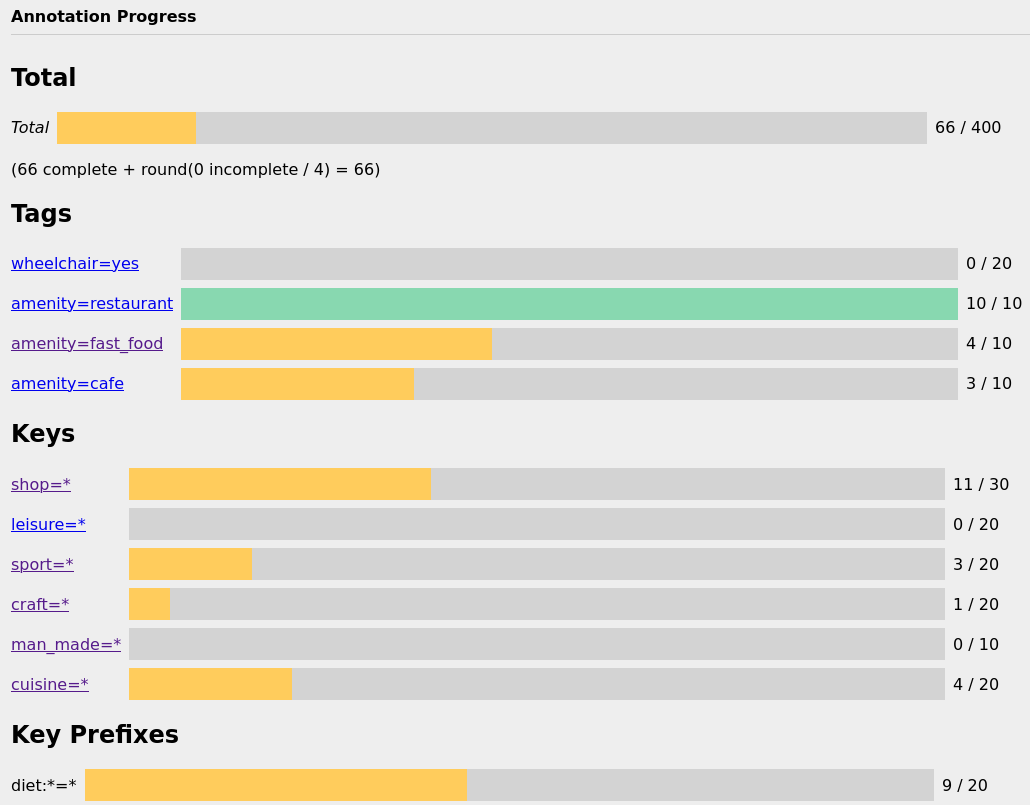
\includegraphics[width=\textwidth]{fig/annotation_progress.png}
  \caption[Annotation progress overview]{Overview of an annotator’s annotation
    progress}
  \label{fig:annotation-progress}
\end{figure}

\section{Online Learning Simulation}
\label{sec:online-simulation}

%%% Local Variables:
%%% coding: utf-8
%%% mode: latex
%%% TeX-engine: xetex
%%% TeX-parse-self: t
%%% TeX-command-extra-options: "-shell-escape"
%%% TeX-master: "../thesis"
%%% End: